% !TeX encoding = UTF-8
% !TeX program = pdflatex
% !TeX spellcheck = it_IT
\documentclass[binding=0.6cm,noexaminfo]{sapthesis}
\usepackage{graphicx}
\usepackage{tikz}
\usepackage{pgfplots}
\usepackage{microtype}
\usepackage[italian]{babel}
\usepackage[utf8]{inputenc}
\usepackage{hyperref}
\usepackage{booktabs, multirow}
\usepackage{amsmath}
\usepackage{amssymb}
\usepackage{threeparttable,booktabs}
%\usepackage{refcheck}
%\nocite{*}
\hypersetup{pdftitle={Un Approccio alla Voice Conversion a Spettro Ridotto attraverso la Sine-Wave Speech},pdfauthor={Davide Gabrielli}}
\title{Un Approccio alla Voice Conversion a Spettro Ridotto attraverso la Sine-Wave Speech}
\author{Davide Gabrielli}
\IDnumber{1883616}
\course{Laurea Triennale in Informatica}
\courseorganizer{Facoltà di Ingegneria dell’Informazione, Informatica e Statistica}
\AcademicYear{2021/2022}
\advisor{Prof. Danilo Avola}
\coadvisor{
	Prof. Luigi Cinque \\
	Dr. Daniele Pannone
}
\authoremail{gabrielli.1883616@studenti.uniroma1.it}
\copyyear{2022}
\thesistype{Tesi di Laurea Triennale}
\begin{document}
	\frontmatter
	\maketitle
	
	\dedication{
		Ai miei genitori e mia sorella,\\
		che mi hanno da sempre supportato\\
		e dovuto ascoltare ogni mia spiegazione non richiesta di tutto questo.\\ \vspace{5mm}
		A Fiorella,\\
		che mi ha insegnato a scrivere in italiano, o che almeno ci ha provato,\\
		e mi ha detto sempre le cose giuste per tranquillizzarmi.\\ \vspace{5mm}
		Ai miei amici,\\
		che mi hanno sostenuto\\
		e dato modo di vedere ogni tanto luci diverse da quelle del monitor.\\ \vspace{5mm}
		Al mio gatto Luna,\\
		che mi ha sempre fatto compagnia nelle notti insonni a scrivere\\
		(a differenza di Maya che se la dormiva).
	}
	\begin{abstract}
	L'idea per cui sia possibile disaccoppiare il contenuto linguistico dall'identità vocale è ricorrente all'interno di varie aree dello speech processing. Si può infatti considerare la voce come la somma di due componenti: una acustica, dipendente dall'interlocutore, e una linguistica, indipendente dall'interlocutore.
	
	Questa tesi ha lo scopo di introdurre nel campo della voice conversion un approccio che sfrutti codifiche audio a spettro ridotto al fine di ridurre la componente acustica. Per tale scopo verranno impiegate delle rappresentazioni in sine-wave speech e in vocoded speech, che in letteratura scientifica hanno dimostrato di preservare l'intelligibilità nonostante la forte alterazione dello spettro sonoro.	
	\end{abstract}
	\tableofcontents
	\mainmatter
	
	\chapter{Introduzione}
		In questo capitolo si farà un'introduzione sull'importanza della voce, ponendo attenzione su cosa si intende per voice conversion e su cosa può comportare lo sviluppo di tali tecniche. Verrà inoltre analizzato lo stato dell'arte e descritto cosa si andrà a realizzare nell'ambito di questa tesi.
	
		\section{Ambito e scopo dell'applicazione}
			La voce è uno strumento comunicativo di cruciale importanza nelle relazioni umane in quanto ci consente di esprimere pensieri e di condividere informazioni con altri individui. Tuttavia essa non è unicamente informazione verbale, infatti oltre ad essere un veicolo per il contenuto linguistico che vogliamo esprimere è caratterizzata anche da aspetti acustici, come timbrica e intonazione.
			Queste ultime sono fondamentali poiché ci permettono di distinguere l’identità a cui corrisponde una determinata voce, tema che anch'esso ha sollevato recentemente molto interesse nel campo della ricerca sulla \textit{speaker recognition}\cite{speaker-recognition}.
			
			Con il termine \textit{voice conversion} si fa riferimento a tutte quelle tecniche che permettono di trasformare la voce di una persona \textit{sorgente} in un’altra voce \textit{target} preservando il contenuto linguistico, ovvero andando a modificare unicamente le caratteristiche dipendenti dall'interlocutore (come formanti, frequenza fondamentale, intonazione, intensità e durata) mantenendo invece quelle indipendenti che rappresentano il contenuto effettivo.
			
			La procedura tipica di VC si può riassumere in tre fasi fondamentali (Fig. \ref{fig:vc-pipeline})\cite{voice-conversion-overview}:
			\begin{enumerate}
				\item \textbf{Analisi}: Si ottiene una rappresentazione intermedia del segnale originale che sia più facilmente manipolabile o che renda più semplice l'estrazione di feature.
				\item \textbf{Trasformazione}: Si crea una mappatura tra le caratteristiche del segnale sorgente e quelle del segnale target e lo si trasforma.
				\item \textbf{Ricostruzione}: Si inverte la rappresentazione intermedia, a cui è stata applicata la trasformazione, al fine di ottenere il risultato finale come audio riproducibile.
			\end{enumerate}
			Risulta interessante notare come la VC non sia esclusivamente l'applicazione di una trasformazione ad un segnale ma includa anche delle rappresentazioni intermedie, il cui ruolo è cruciale in quanto potrebbero facilitare le operazioni di mappatura oppure causare artefatti e comprometterne il risultato.
			\begin{figure}%[h]
				\centering
				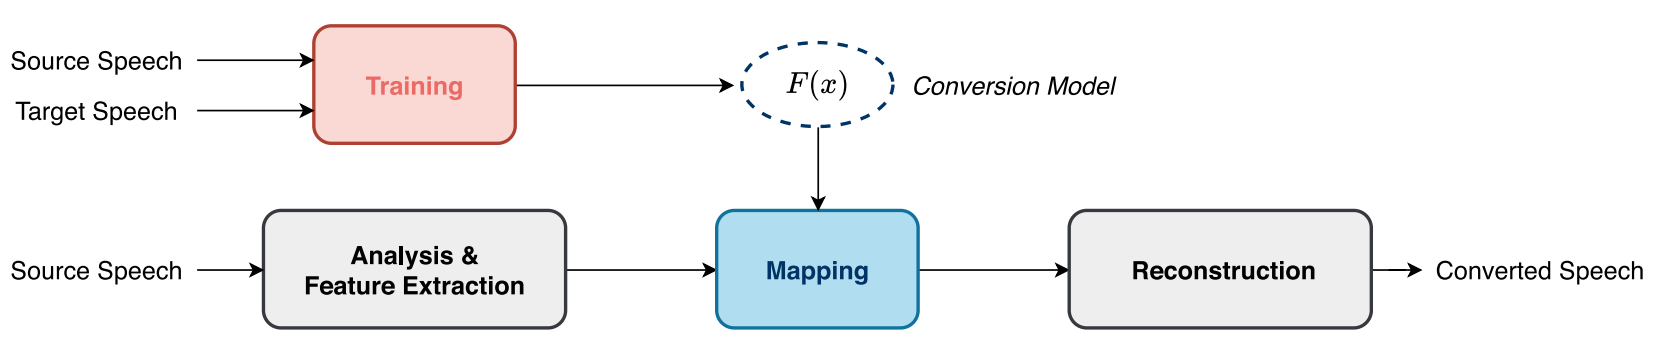
\includegraphics[width=1\linewidth]{figures/vc-pipeline}
				\caption{Pipeline tipica della voice conversion. Fonte \cite{voice-conversion-overview}.}
				\label{fig:vc-pipeline}
			\end{figure}
			L’interesse per la VC è dato dall’applicazione in vari campi come: sintesi vocale personalizzata, anonimizzazione voce e mimica vocale.
			Il tema è oggetto di ricerca nel campo della sintesi vocale e recentemente, grazie all’impiego di tecniche di deep learning, sono stati ottenuti importanti progressi. 
	
		\section{Stato dell'arte}
			In questa sezione si riporta una classificazione dei metodi per la voice conversion che impiegano tecniche di deep learning, estratta dall'analisi svolta da Sisman et al.\cite{voice-conversion-overview}, distinguendo in due categorie differenti in base alla tipologia del dataset impiegato nella fase di training: impiego di dati paralleli e impiego di dati non paralleli.
			
			\subsection{Dati paralleli}
			I primi studi si sono focalizzati sull'impiego di dati paralleli, vale a dire impiegando dataset formati da audio di parole, o frasi, pronunciati da entrambi gli speaker dei quali si vuole la conversione. Il task è piuttosto semplice poiché avendo a disposizione audio corrispondenti e allineati, il problema si riduce a creare una mappatura tra questi.
			
			Tuttavia ciò può risultare complesso e sebbene il problema dell'allineamento degli audio possa essere ovviato mediante l'impiego di encoder-decoder con meccanismo di attention\cite{attention-mechanism}, rimane comunque la problematica di avere a disposizione tali dati.
			
			\subsection{Dati non paralleli}
			Studi recenti hanno mostrato come siano possibili conversioni di voci anche con dati non paralleli, ovvero impiegando dataset che non presentano alcun audio di parole, o frasi, pronunciati da entrambi gli speaker di cui si vuole la conversione.
			
			In base all'approccio usato per realizzare ciò si possono distinguere quattro categorie principali:
			\begin{enumerate}
				\item Dati non paralleli di una coppia di speaker definita
				\item Impiego di sistemi Text-to-Speech
				\item Impiego di sistemi di Automated Speech Recognition
				\item Separazione del contenuto linguistico dallo speaker
			\end{enumerate}
			Si procede dunque con un'analisi di quelle che sono le tecniche allo stato dell'arte per ciascuno di essi.
			
			\paragraph{1) Dati non paralleli di una coppia di speaker definita}
			Le tecniche attualmente impiegate per la voice conversion con dati non paralleli di una coppia di speaker definita sono le stesse impiegate nell'\textit{image-to-image translation}, il cui obiettivo è trovare una mappatura da un dominio $X$ ad un dominio $Y$ mantenendone la struttura.
			Infatti come nella image translation si può volere, ad esempio, convertire fotografie di paesaggi in quadri di Monet, mantenendone il contesto originale rappresentato, così nella conversione di voci si vuole trasformare la voce tra due speaker differenti mantenendone il contenuto linguistico.
			
			Allo stato dell'arte abbiamo la CycleGAN-VC\cite{CycleGAN2017} proposta da Kaneko et al., in particolare con le sue varianti CycleGAN-VC2\cite{CycleGAN-VC2}, CycleGAN-VC3\cite{CycleGAN-VC3} e MaskCycleGAN-VC\cite{MaskCyclegan-VC} che verranno approfondite nel \autoref{chap:deep-learning}.
			
			\paragraph{2) Impiego di sistemi Text-to-Speech}
			Uno degli aspetti importanti della voice conversion è preservare il contenuto linguistico dalla voce sorgente a quella di destinazione, la quale è una caratteristica in comune con i sistemi Text-to-Speech (TTS) capaci di generare audio sintetico partendo da trascrizioni date. Questi ultimi si basano principalmente su modelli encoder-decoder e pertanto risulta possibile sfruttarli per la conversione attraverso tecniche di transfer learning\cite{transfer-learning-tts-vc}, condividendo la parte del decoder. Tuttavia la maggior parte di questi approcci richiede molti dati per la fase di addestramento del modello di TTS che non sempre sono disponibili.
			
			\paragraph{3) Impiego di sistemi Automated Speech Recognition}
			Gli approcci basati sul deep learning per la voice conversion richiedono grandi quantità di dati al fine di poter creare una rappresentazione latente che descriva il sistema fonetico.
			
			Tuttavia sappiamo che la maggior parte dei sistemi di riconoscimento automatico del parlato (ASR) sono già stati addestrati su grandi dati e descrivono correttamente il sistema fonetico, pertanto risulta interessante sfruttare la rappresentazione latente di essi nella conversione di voci.
			
			Un approccio particolarmente di successo consiste nel costruire un modello che sfrutti i phonetic posteriogram (PPG) estratti da un sistema di SI-ASR (speaker-independent ASR) al fine di creare una mappatura verso una voce target\cite{ppg-vc}.
			
			\paragraph{4) Separazione del contenuto linguistico dallo speaker}
			Per separare il contenuto linguistico dallo speaker sono possibili vari approcci, tra i più efficaci si menzionano l'impiego di instance normalization\cite{instance-normalization}, vector quantization\cite{vector-quantization} e l'utilizzo di auto-encoder\cite{auto-encoder}.
			
			Un auto-encoder impara a riprodurre l'output come il suo input, e per tale scopo deve costruire una rappresentazione latente intermedia. Questa codifica interna può essere vista come una forma compressa dell'input che mantiene tutte le informazioni necessarie per ricostruire il segnale originale in output.
			Questi approcci tuttavia tendono a generare audio di bassa qualità per via dell'eccessiva rimozione di informazione.
	
		\section{Contributo}
			Questo lavoro ha lo scopo di esplorare la conversione di voci con riduzione dello spettro sonoro. Partendo dall'idea per cui è possibile da un audio di una voce disaccoppiare la componente linguistica (indipendente dallo speaker) da quella acustica (dipendente dallo speaker), si vuole trovare una rappresentazione che riduca le caratteristiche di quest'ultima senza l'impiego di ulteriori dati o modelli pre-trained.
			
			Per fare ciò sono state impiegate tecniche tradizionali di speech processing per il pre-processamento dei dati, ottenendo così delle rappresentazioni in \textit{sine-wave speech}, \textit{buzz vocoded} e \textit{noise vocoded} degli stessi. Questi sono poi stati impiegati per addestrare un modello di tipo MaskCycleGAN-VC\cite{MaskCyclegan-VC}, stato dell'arte per quanto riguarda la voice conversion con dati non paralleli di coppie di speaker, e ne sono stati confrontati i risultati.
	
	
	\chapter{Audio}
		In questo capitolo verrà descritto il suono, le sue caratteristiche e le sue rappresentazioni digitali, partendo dalle più comuni fino ad arrivare a quelle utilizzate per questo lavoro.
		
		\section{Il suono}
			Il suono è un segnale acustico prodotto dalle vibrazioni di un corpo e dalla trasmissione di queste attraverso un mezzo, ad esempio l’aria. Di questo segnale è possibile misurare l’intensità, ovvero la variazione di pressione, l'unità di misura più comunemente utilizzata sono i decibel (dB).
			
			Possiamo dividere i suoni in due classi: periodici e aperiodici.
			Per quanto riguarda i suoni periodici questi possono essere semplici, come delle onde sinusoidali, o complessi, risultato di più onde sinusoidali combinate.
			Mentre i suoni aperiodici non presentano pattern ripetitivi e possono essere continui, come il rumore, o transienti, come impulsi.
			
		\section{Onda sinusoidale}
			Al fine di poter descrivere al meglio cos'è il suono, è necessario definirlo nella sua forma più semplice: l'onda sinusoidale. Essa consiste in un suono periodico semplice, descrivibile con la seguente formula:
			\begin{equation}
				y(t) = A \cdot sin(2 \pi ft + \varphi)
			\end{equation}
			I parametri fondamentali al fine di caratterizzare un'onda sinusoidale dunque sono:
			\begin{enumerate}
				\item \textbf{Frequenza} (f): La frequenza di un suono è un concetto che si basa sulla periodicità di un segnale ed è espresso come l'inverso del tempo che esso impiega a ripetersi, ovvero a compiere un ciclo ($f=1/T$).
				\item \textbf{Ampiezza} (A): L'ampiezza di un segnale è la misurazione della variazione di pressione dello stesso.
				\item \textbf{Fase} ($\varphi$): La fase di un segnale rappresenta la quantità di frazione di un ciclo, quindi una completa oscillazione, compiuta dall'onda.
			\end{enumerate}
			
		\section{Digitalizzazione segnale audio}
			Al fine di poter rappresentare digitalmente questi segnali analogici, abbiamo bisogno di un campionamento (Fig. \ref{fig:campionamento}).
			Esso consiste nel misurare e registrare la pressione sonora del segnale acustico ogni T secondi, tale valore viene definito come \textit{intervallo di campionamento}. Il numero di campioni che registriamo in un secondo viene definita \textit{frequenza di campionamento}.
			
			Il teorema di Nyquist-Shannon definisce la frequenza massima rappresentabile $f_{N}$ (frequenza di Nyquist) dato un campionamento con una frequenza $f_{s}$ senza perdita di informazione.
			\begin{equation}
				f_{N} = \frac{1}{2} f_{s}
				\label{eq:fn}
			\end{equation}
			
			Nonostante questa tipologia di codifica dell'audio risulti ottimale per la conversione analogico-digitale dei segnali, non ci permette agilmente di ottenere quelle che sono le feature più interessanti per la nostra percezione.
			\begin{figure}%[h]
	\centering
	\begin{tikzpicture}[>=latex]
		\begin{axis}[
			axis lines = middle,
			xlabel = Tempo,
			ylabel = Ampiezza,
			xtick={0,1,...,25},
			ytick={-2,-1,...,2},
			xmin=0,
			xmax=25.5,
			ymin=-2.5,
			ymax=2.5,
			width=140mm,
			height=60mm,
			]
			\addplot[
			scatter,
			domain=0:25,
			samples=40,
			color=black
			]
			{sin(180*x/6)+cos(180*x/8)};
			\addplot[
			only marks,
			domain=0:25,
			samples=40,
			color=blue
			]{sin(180*x/6)+cos(180*x/8)};
			\addplot[
			ycomb,
			dashed,
			domain=0:25,
			samples=40,
			color=blue
			]
			{sin(180*x/6)+cos(180*x/8)};
		\end{axis}
	\end{tikzpicture}
	\caption{Campionamento di un segnale audio complesso. L'onda viene scomposta in campioni equidistanti che rappresentino l'ampiezza nel tempo, descrivendo l'onda originale.}
	\label{fig:campionamento}
\end{figure}
			
		\section{Spettrogramma}
		Uno spettrogramma è una rappresentazione dello spettro di potenza di un segnale audio sul dominio del tempo (Fig. \ref{fig:spettrogramma}). Al fine di definire uno spettrogramma, è dunque necessario prima descrivere cosa sia uno spettro di potenza. Esso consiste nella rappresentazione di un segnale audio in un certo istante temporale $t$ in funzione della frequenza.
				
		Il metodo più veloce per calcolare lo spettro di potenza di un segnale audio è attraverso la \textit{fast Fourier transform} (FFT), un algoritmo che calcola la \textit{trasformata discreta di Fourier} (DFT) con costo computazionale $O(n \cdot log(n))$\cite{audio-fft}.
		\begin{figure}[h]
			\centering
			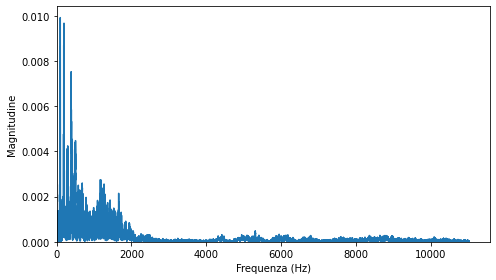
\includegraphics[width=0.75\linewidth]{figures/spectrum}
			\caption{Spettro di potenza di una voce maschile pronunciando "It's not forever".}
			\label{fig:spettro}
		\end{figure}
		Calcolando la DFT sull'intero audio otteniamo dunque lo spettro dell'intero segnale audio analizzato (Fig. \ref{fig:spettro}) ma non possiamo sapere in quale istante sono avvenuti i principali picchi.
		
		Per ovviare a questo problema di mancanza di riferimento temporale, dobbiamo calcolare la DFT su porzioni di audio in sequenza temporale. Questa operazione viene definita \textit{short-time fourier transform} (STFT) e possiamo così visualizzarne il risultato sotto forma di spettrogrammi (Fig. \ref{fig:spettrogramma})\cite{time-frequency-review}.
		
		 Uno spettrogramma può essere rappresentato con una heat map in cui gli assi descrivono la frequenza e il tempo, mentre l'intensità sonora è espressa attraverso il colore. Questo tipo di codifica ci permette quindi di accedere ad informazioni più rilevanti riguardo il suono in uno spazio ristretto.
		\begin{figure}%[h]
			\centering
			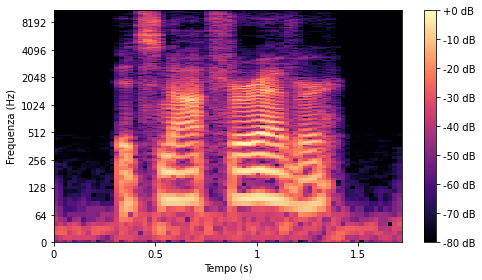
\includegraphics[width=0.75\linewidth]{figures/spectrogram}
			\caption{Spettrogramma di una voce maschile pronunciando "It's not forever".}
			\label{fig:spettrogramma}
		\end{figure}
	
		\section{Spettrogramma mel}
		 Tuttavia è importante considerare come la percezione umana del suono non sia lineare ma sia dipendente dall'altezza sonora (pitch) e quindi dalla frequenza dei suoni che udiamo. La scala mel viene per la prima volta sviluppata nel 1937 in una ricerca effettuata da Stevens e consiste in una scala di frequenze con altezze diverse (pitch) giudicate dagli ascoltatori come equidistanti (Fig. \ref{fig:scala-mel})\cite{Stevens1937}.
		 Non esiste propriamente una formula per la scala di mel ma tra le più comuni troviamo:
		 \begin{equation}
		 	mel(x) = 2595 \log_{10}(1+\frac{x}{700})
		 \end{equation}
		 \newcommand{\vertLineFromPoint}[1]{
	\draw[dashed] 
	(#1) -- (#1|-{rel axis cs:0,0})
}
\newcommand{\horLineFromPoint}[1]{
	\draw[dashed] 
	(#1) -- (#1-|{rel axis cs:0,0})
}
\begin{figure}[h]
	\centering
	\begin{tikzpicture}
		\begin{axis}[
			width=120mm,
			height=58mm,
			axis lines=left,
			domain=0:10000,
			samples=100,
			no markers,
			xlabel=Frequenza (Hz),
			ylabel=Scala Mel (mel),
			y label style={at={(axis description cs:-0.02,.5)}},
			xtick distance=1000,
			ytick distance=250
			]
			\addplot {2595 * log10(1+x/700)};
			\vertLineFromPoint{100,100};
			\horLineFromPoint{100,100};
		\end{axis}
	\end{tikzpicture}
	\caption{Grafico della scala mel.}
	\label{fig:scala-mel}
\end{figure}
	 	
		Possiamo quindi impiegare questa scala per realizzare una rappresentazione che ci consentirà in fase di elaborazione di ottenere manipolazioni più significative per il nostro apparato uditivo (Fig. \ref{fig:spettrogramma-mel}).
		
		L'inversione degli spettrogrammi è soggetta alla produzione di artefatti in quanto nel calcolo della trasformata discreta di Fourier si ha perdita di informazione delle fasi dei segnali. Tuttavia grazie allo sviluppo recente di vocoder neurali, come MelGAN\cite{melgan}, in grado di rigenerare correttamente l'audio a partire da spettrogrammi mel, questi sono diventati sempre più di uso comune.
		\begin{figure}%[h]
			\centering
			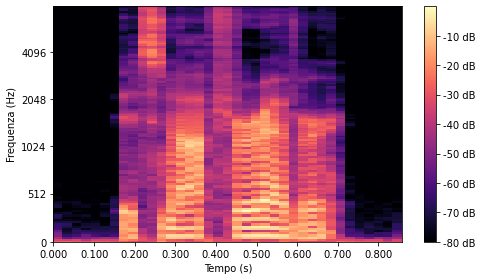
\includegraphics[width=0.75\linewidth]{figures/melspectrogram}
			\caption{Spettrogramma mel di una voce maschile pronunciando "It's not forever".}
			\label{fig:spettrogramma-mel}
		\end{figure}
	
		\section{Coefficienti mel-frequency cepstrum}
		I coefficienti mel-frequency cepstrum (MFCC)\cite{mel-frequency-cepstral} sono una rappresentazione dell'audio largamente usato nello speech processing tradizionale che ha trovato largo utilizzo anche nel machine learning, come nella speech recognition. Al fine di ottenere un MFCC è sufficiente calcolare la \textit{trasformata discreta del coseno} (DCT) dello spettrogramma mel dell'audio desiderato (Fig. \ref{fig:mfcc}).
		\begin{figure}%[h]
			\centering
			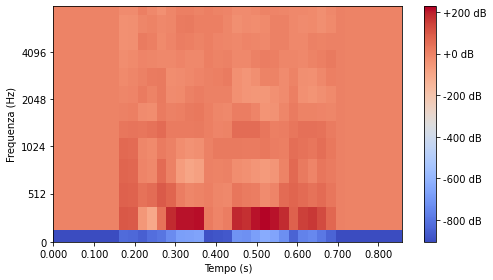
\includegraphics[width=0.75\linewidth]{figures/mfcc}
			\caption{MFCC di una voce maschile pronunciando "It's not forever".}
			\label{fig:mfcc}
		\end{figure}
		
		\section{Sine-wave speech}
		La sine-wave speech (SWS) è una forma di audio del parlato umano a spettro ridotto, in cui vi sono presenti in genere tre o quattro componenti sinusoidali mobili (Fig. \ref{fig:sine-wave-speech}). L'audio viene generato rimpiazzando le formanti con delle sinusoidi al fine di rimuovere il più possibile la componente acustica mantenendo però intelligibilità.
		\begin{figure}[h]
			\centering
			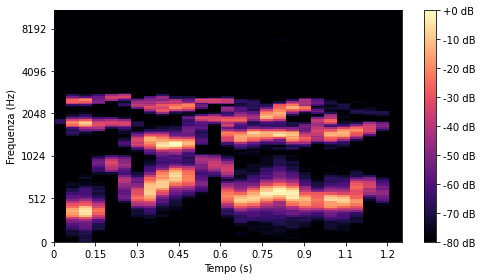
\includegraphics[width=0.75\linewidth]{figures/sine-wave_speech}
			\caption{Spettrogramma mel di una voce maschile pronunciando "It's not forever" in SWS con 3 componenti.}
			\label{fig:sine-wave-speech}
		\end{figure}
	
		Viene per la prima volta sviluppato negli Haskins Laboratories da Rubin\cite{haskins-laboratories} e successivamente impiegato in vari esperimenti riguardanti la percezione del parlato, come da Remez et al. che nel 1981 dimostrò come nonostante la sua apparente forma innaturale, la sine-wave speech conservi le proprietà sufficienti per la percezione del contenuto linguistico\cite{remez1981speech}.
		
		\section{Vocoded speech}
		Il vocoder è una tecnica di elaborazione dell'audio che richiede due sorgenti: un carrier, che accoglierà il suono, e un modulatore, che darà forma al suono del carrier. Le caratteristiche armoniche del modulatore vengono codificate all'interno del carrier, ottenendo un segnale con uno spettro alterato (Fig. \ref{fig:buzz-vocoded} e \ref{fig:noise-vocoded}).
		
		Le ricerche sulla percezione del parlato in condizioni di alterazione spettrale trovano il loro interesse anche per questa forma di modulazione. Il lavoro di Davis et al. sulla comprensione del parlato noise-vocoded dimostra come anche in questo caso, l'ascoltatore impari a riconoscere il parlato nonostante la forte distorsione di esso\cite{noise-vocoded}.
		\begin{figure}%[h]
			\centering
			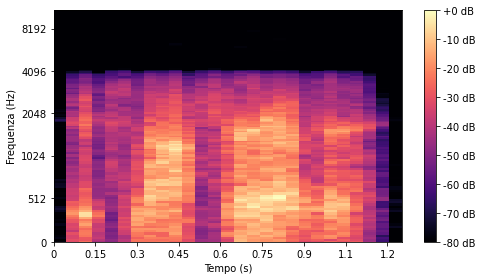
\includegraphics[width=0.75\linewidth]{figures/noise-vocoded}
			\caption{Vocoder con noise come carrier e una voce maschile pronunciando "It's not forever" come modulatore.}
			\label{fig:noise-vocoded}
		\end{figure}
		\begin{figure}%[h]
			\centering
			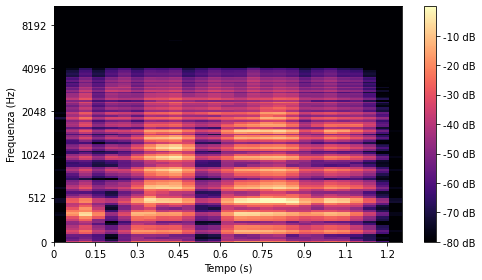
\includegraphics[width=0.75\linewidth]{figures/buzz-vocoded}
			\caption{Vocoder con un buzz a 500 Hz come carrier e una voce maschile pronunciando "It's not forever" come modulatore.}
			\label{fig:buzz-vocoded}
		\end{figure}
	
	
	\chapter{Deep Learning}
	\label{chap:deep-learning}
		In questo capitolo sarà introdotto il deep learning, verranno descritte architetture di reti neurali semplici fino ad arrivare ad alcune più complesse utilizzate in questo lavoro.
		
		\section{Introduzione}
		Il deep learning è una branca del machine learning che si basa sull'apprendimento della rappresentazione dei dati. A differenza dei tipici approcci in cui si scrive un algoritmo per svolgere un'attività specifica, si realizzano invece degli algoritmi in grado di imparare a mappare dati tra domini differenti.
		Questa disciplina prende forte ispirazione dall'organizazione del cervello che, attraverso diverse trasformazioni e rappresentazioni, riesce ad imparare a processare le informazioni.
		
		\section{Percettrone}
		Un percettrone è l'architettura neurale minima, introdotta nel 1958 da Rosenblatt\cite{perceptron}, ed è ispirata al funzionamento del neurone, unità minima del cervello umano. Esattamente come un neurone esso infatti riceve dei segnali di ingresso e applica una somma pesata come segue:
		\begin{equation}
			y = w_0 + \sum_{i=1}^n x_i w_i
		\end{equation}
		L'output $y$ viene poi passato ad una funzione di attivazione che deciderà se il percettrone deve attivarsi o meno.
		\usetikzlibrary{positioning}
\tikzset{basic/.style={draw,fill=blue!20,text width=1.2em,text badly centered}}
\tikzset{input/.style={basic,circle}}
\tikzset{weights/.style={basic,rectangle}}
\tikzset{functions/.style={basic,circle,fill=blue!10}}
\begin{figure}%[h]
	\centering
	\begin{tikzpicture}
		\node[functions] (center) {};
		\node[below of=center,font=\scriptsize,text width=4em] {Funzione di attivazione};
		\draw[thick] (0.5em,0.5em) -- (0,0.5em) -- (0,-0.5em) -- (-0.5em,-0.5em);
		\node[right of=center] (right) {};
		\path[draw,->] (center) -- (right);
		\node[functions,left=3em of center] (left) {$\sum$};
		\path[draw,->] (left) -- (center);
		\node[weights,left=3em of left] (2) {$w_2$} -- (2) node[input,left of=2] (l2) {$x_2$};
		\path[draw,->] (l2) -- (2);
		\path[draw,->] (2) -- (left);
		\node[below of=2] (dots) {$\vdots$} -- (dots) node[left of=dots] (ldots) {$\vdots$};
		\node[weights,below of=dots] (n) {$w_n$} -- (n) node[input,left of=n] (ln) {$x_n$};
		\path[draw,->] (ln) -- (n);
		\path[draw,->] (n) -- (left);
		\node[weights,above of=2] (1) {$w_1$} -- (1) node[input,left of=1] (l1) {$x_1$};
		\path[draw,->] (l1) -- (1);
		\path[draw,->] (1) -- (left);
		\node[weights,above of=1] (0) {$w_0$} -- (0) node[input,left of=0] (l0) {$1$};
		\path[draw,->] (l0) -- (0);
		\path[draw,->] (0) -- (left);
		\node[below of=ln,font=\scriptsize] {Input};
		\node[below of=n,font=\scriptsize] {Pesi};
	\end{tikzpicture}
	\caption{Un percettrone con una funzione di attivazione sull'output.}
\end{figure}
		
		\section{Funzione di attivazione}
		Una funzione di attivazione è una trasformazione non lineare applicata all'output di un percettrone al fine di mapparlo in un range di valori differente.
		Si descrivono a seguire alcune delle più note funzioni di attivazione.
		\paragraph{Sigmoid}
		La funzione Sigmoid (Fig. \ref{fig:sigmoid}) è stata storicamente la più usata tra le funzioni di attivazione. Essa offre il vantaggio di mappare i valori nell'intervallo (0,1).
		\[ \sigma(z) = \frac{1} {1 + e^{-z}} \]
		\begin{figure}%[h]
			\centering
			\begin{tikzpicture}[
				declare function={sigma(\x)=1/(1+exp(-\x));
				sigmap(\x)=sigma(\x)*(1-sigma(\x));}]
				\begin{axis}%
					[
					width=4in,
					height=2in,
					grid=major, 
					xmin=-5,
					xmax=5,
					axis x line=bottom,
					ytick={0,.5,1},
					ymax=1,
					axis y line=middle,
					samples=100,
					domain=-5:5,
					legend style={at={(0.05,0.9)},anchor=north west}
					]
					\addplot[blue,mark=none] (x,{sigma(x)});
					\addplot[red,mark=none] (x,{sigmap(x)});
					\legend{$\sigma(x)$,$\sigma'(x)$}
				\end{axis}
			\end{tikzpicture}
			\caption{Grafico della funzione Sigmoid.}
			\label{fig:sigmoid}
		\end{figure}
		
		\paragraph{Tanh}
		La funzione Tanh (Fig. \ref{fig:tanh}) è anch'essa sigmoidea. La principale differenza che la distingue da Sigmoid è che il suo dominio di output è in (-1,1)  che la rende particolarmente adatta nei problemi di classificazione con due classi.
		\[ tanh(x) = \frac{e^x - e^{-x}}{e^x + e^{-x}} = \frac{1 - e^{-2x}}{1 + e^{-2x}} \]
		\begin{figure}%[h]
		\centering
		\begin{tikzpicture}
			\begin{axis}%
				[
				width=4in,
				height=2in,
				grid=major,
				xmin=-5,
				xmax=5,
				axis x line=center,
				ymax= 1,
				ymin= -1,
				axis y line=middle,
				samples=500,
				domain=-5:5,
				legend style={at={(0.05,0.9)},anchor=north west}
				]
				\addplot[blue,mark=none] (x,{tanh(x)});
				\addplot[red,mark=none] (x,{1-(tanh(x)*tanh(x))});
				\legend{$tanh(x)$,$tanh'(x)$}
			\end{axis}
		\end{tikzpicture}
		\caption{Grafico della funzione Tanh.}
		\label{fig:tanh}
		\end{figure}
		
		\paragraph{ReLU}
		La funzione ReLU (Fig. \ref{fig:relu}) è il nuovo standard per molti tipi di reti neurali in quanto permette di abbassare notevolmente il costo computazionale dell'addestramento del modello. Essa è una funzione lineare definita a tratti, che mappa in zero tutti i numeri negativi e gli altri nell'input stesso\cite{ReLU}.
		\[ ReLU(z) = max(0, z) \]
		\begin{figure}%[h]
			\centering
			\begin{tikzpicture}
				\begin{axis}%
					[
					width=4in,
					height=2in,
					grid=major, 
					xmin=-5,
					xmax=5,
					axis x line=bottom,
					ymax= 4,
					axis y line=middle,
					samples=500,
					domain=-5:5,
					legend style={at={(0.05,0.9)},anchor=north west}
					]
					\addplot[blue,mark=none] (x,{max(0,x)});
					\addplot[red,mark=none] (x,{(x>0)});
					\legend{$ReLU(x)$,$ReLU'(x)$}
				\end{axis}
			\end{tikzpicture}
			\caption{Grafico della funzione ReLU.}
			\label{fig:relu}
		\end{figure}
		
		\section{Rete neurale artificiale}
		I percettroni sono solitamente organizzati in livelli, che possono avere strutture diverse per effettuare trasformazioni differenti. Una rete neurale artificiale (ANN) è formata da più livelli interconnessi e organizzati come segue:
		\begin{itemize}
			\item \textbf{Livello di input}: ottiene i dati iniziali per la rete neurale.
			\item \textbf{Livelli nascosti}: livelli intermedi che svolgono la computazione.
			\item \textbf{Livello di output}: produce il risultato finale.
		\end{itemize}
		Il tipo di ANN più semplice è una Multilayer Perceptron (MLP), un'architettura fully connected e feedforward, ovvero in cui ogni nodo in uscita è connesso ad ogni altro nodo del livello successivo (Fig. \ref{fig:mlp}).
		% !TeX encoding = UTF-8
% !TeX program = pdflatex
% !TeX spellcheck = it_IT
\usetikzlibrary{positioning}
\tikzset{%
	every neuron/.style={
		circle,
		draw,
		minimum size=1cm
	},
	neuron missing/.style={
		draw=none, 
		scale=2,
		text height=0.333cm,
		execute at begin node=\color{black}$\vdots$
	},
}
\begin{figure}[h]
\centering
\begin{tikzpicture}[x=1.5cm, y=1.2cm, >=stealth]
	
	\foreach \m/\l [count=\y] in {1,2,3,missing,4}
	\node [every neuron/.try, neuron \m/.try] (input-\m) at (0,2.5-\y) {};
	
	\node [every neuron/.try, neuron 1/.try ] (hidden-1) at (2, 1.25) {};
	\node [every neuron/.try, neuron missing/.try ] (hidden-missing) at (2, 0.1*1.25) {};
	\node [every neuron/.try, neuron 1/.try ] (hidden-2) at (2, -1*1.25) {};	
	
	\foreach \m [count=\y] in {1,missing,2}
	\node [every neuron/.try, neuron \m/.try ] (output-\m) at (4,1.5-\y) {};
	
	\foreach \l [count=\i] in {1,2,3,n}
	\draw [<-] (input-\i) -- ++(-1,0)
	node [above, midway] {$I_\l$};
	
	\foreach \l [count=\i] in {1,n}
	\node [above] at (hidden-\i.north) {$H_\l$};
	
	\foreach \l [count=\i] in {1,n}
	\draw [->] (output-\i) -- ++(1,0)
	node [above, midway] {$O_\l$};
	
	\foreach \i in {1,...,4}
	\foreach \j in {1,...,2}
	\draw [->] (input-\i) -- (hidden-\j);
	
	\foreach \i in {1,...,2}
	\foreach \j in {1,...,2}
	\draw [->] (hidden-\i) -- (output-\j);
	
	\foreach \l [count=\x from 0] in {di input, nascosto, di output}
	\node [align=center, above] at (\x*2,2) {Livello \\ \l};
	
\end{tikzpicture}
\caption{Grafo rappresentante una MLP.}
\label{fig:mlp}
\end{figure}
		
		\section{Algoritmi di apprendimento}
		Gli algoritmi di machine learning si possono suddividere in tre categorie in base alle modalità di svolgimento della fase di addestramento\cite{deep-learning-book}:
		\begin{itemize}
			\item \textbf{Supervised Learning}: paradigma applicabile laddove sia presente un dataset con elementi che abbiano un'etichetta applicata o che abbiano un corrispondente elemento obiettivo, utile ai fini di classificazione o regressione.
			\item \textbf{Unsupervised Learning}: paradigma applicabile laddove sia utile imparare proprietà sulla struttura dei dati, come per la generazione o la riduzione del rumore da essi.
			\item \textbf{Semi-supervised Learning}: sfrutta sia tecniche del supervised learning, sia dell'unsupervised learning. Nello specifico si sfrutta la conoscenza fornita dai dati etichettati per classificare anche i restanti. Questa tecnica agevola la costruzione del dataset in quanto si possono usare più dati ma richiede comunque una prevalenza di dati etichettati.
		\end{itemize}
		
		\section{Reti neurali avanzate}
		In questa sezione vengono descritte le principali reti neurali avanzate utilizzate in questo lavoro.
		
		\subsection{CNN}
		Una CNN (Convolutional Neural Network) è una tipologia di rete neurale artificiale comunemente utilizzata nella classificazione di immagini (Fig. \ref{fig:cnn})\cite{cnn}. La rete è composta in genere da tre tipi di livelli:
		\begin{itemize}
			\item \textbf{Livelli convoluzionali}: applicano dei filtri alle immagini al fine di estrarre feature da esse.
			\item \textbf{Livelli di pooling}: riducono lo spazio di rappresentazione raccogliento output vicini basandosi su calcoli statistici come media o massimo.
			\item \textbf{Livelli fully connected}: connettono tutti i nodi tra loro in modo da poter permettere la classificazione basandosi sulle feautre estratte. 
		\end{itemize}
		\begin{figure}[h]
			\centering
			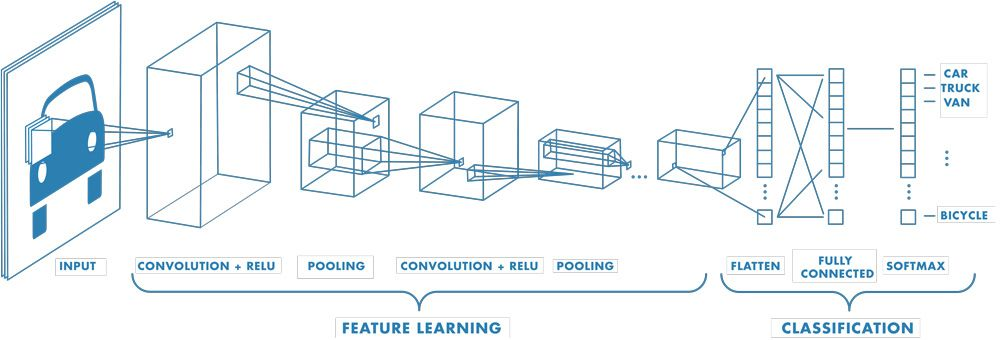
\includegraphics[width=0.7\linewidth]{figures/CNN}
			\caption{Convolutional Neural Network per la classificazione di immagini. Fonte https://it.mathworks.com/discovery/convolutional-neural-network-matlab.html.}
			\label{fig:cnn}
		\end{figure}
		
		\subsection{GAN}
			Una GAN (Generative Adversarial Network) è una classe di algoritmi di deep learning proposta nel 2014 da Goodfellow\cite{Goodfellow}. Consiste in due reti neurali che competono in un gioco a somma zero (\ref{eq:gan}), addestrando due modelli allo stesso tempo: un modello generativo (G) e un modello discriminatore (D).
			La rete generativa produrrà immagini che verranno passate in input alla rete discriminatore mentre quest'ultima si occuperà di classificarle come reali o generate (Fig. \ref{fig:gans}).
			\begin{equation}
				\min_G\max_D{V(D, G)} = \min_G\max_D \left[\; \mathbb{E}_{x \sim p_{data}}[log \; D(x)] + \; \mathbb{E}_{z \sim p_{z}}[log \; (1 - D(G(z)))] \right]
				\label{eq:gan}
			\end{equation}
			
			Il discriminatore è un classificatore che impara a distinguere dati reali da quelli creati dal generatore, questo sarà addestrato usando dati reali e l'output del generatore, e verrà penalizzato in caso classifichi scorrettamente i dati e aggiornando i suoi pesi attraverso backpropagation.
			
			Il generatore è una rete che impara a generare immagini false che sembrino realistiche, questo sarà addestrato usando dati casuali e il suo output verrà collegato al discriminatore, e verrà penalizzato in caso esso rilevi l'immagine generata come falsa.
			
			\begin{figure}[h]
				\centering
				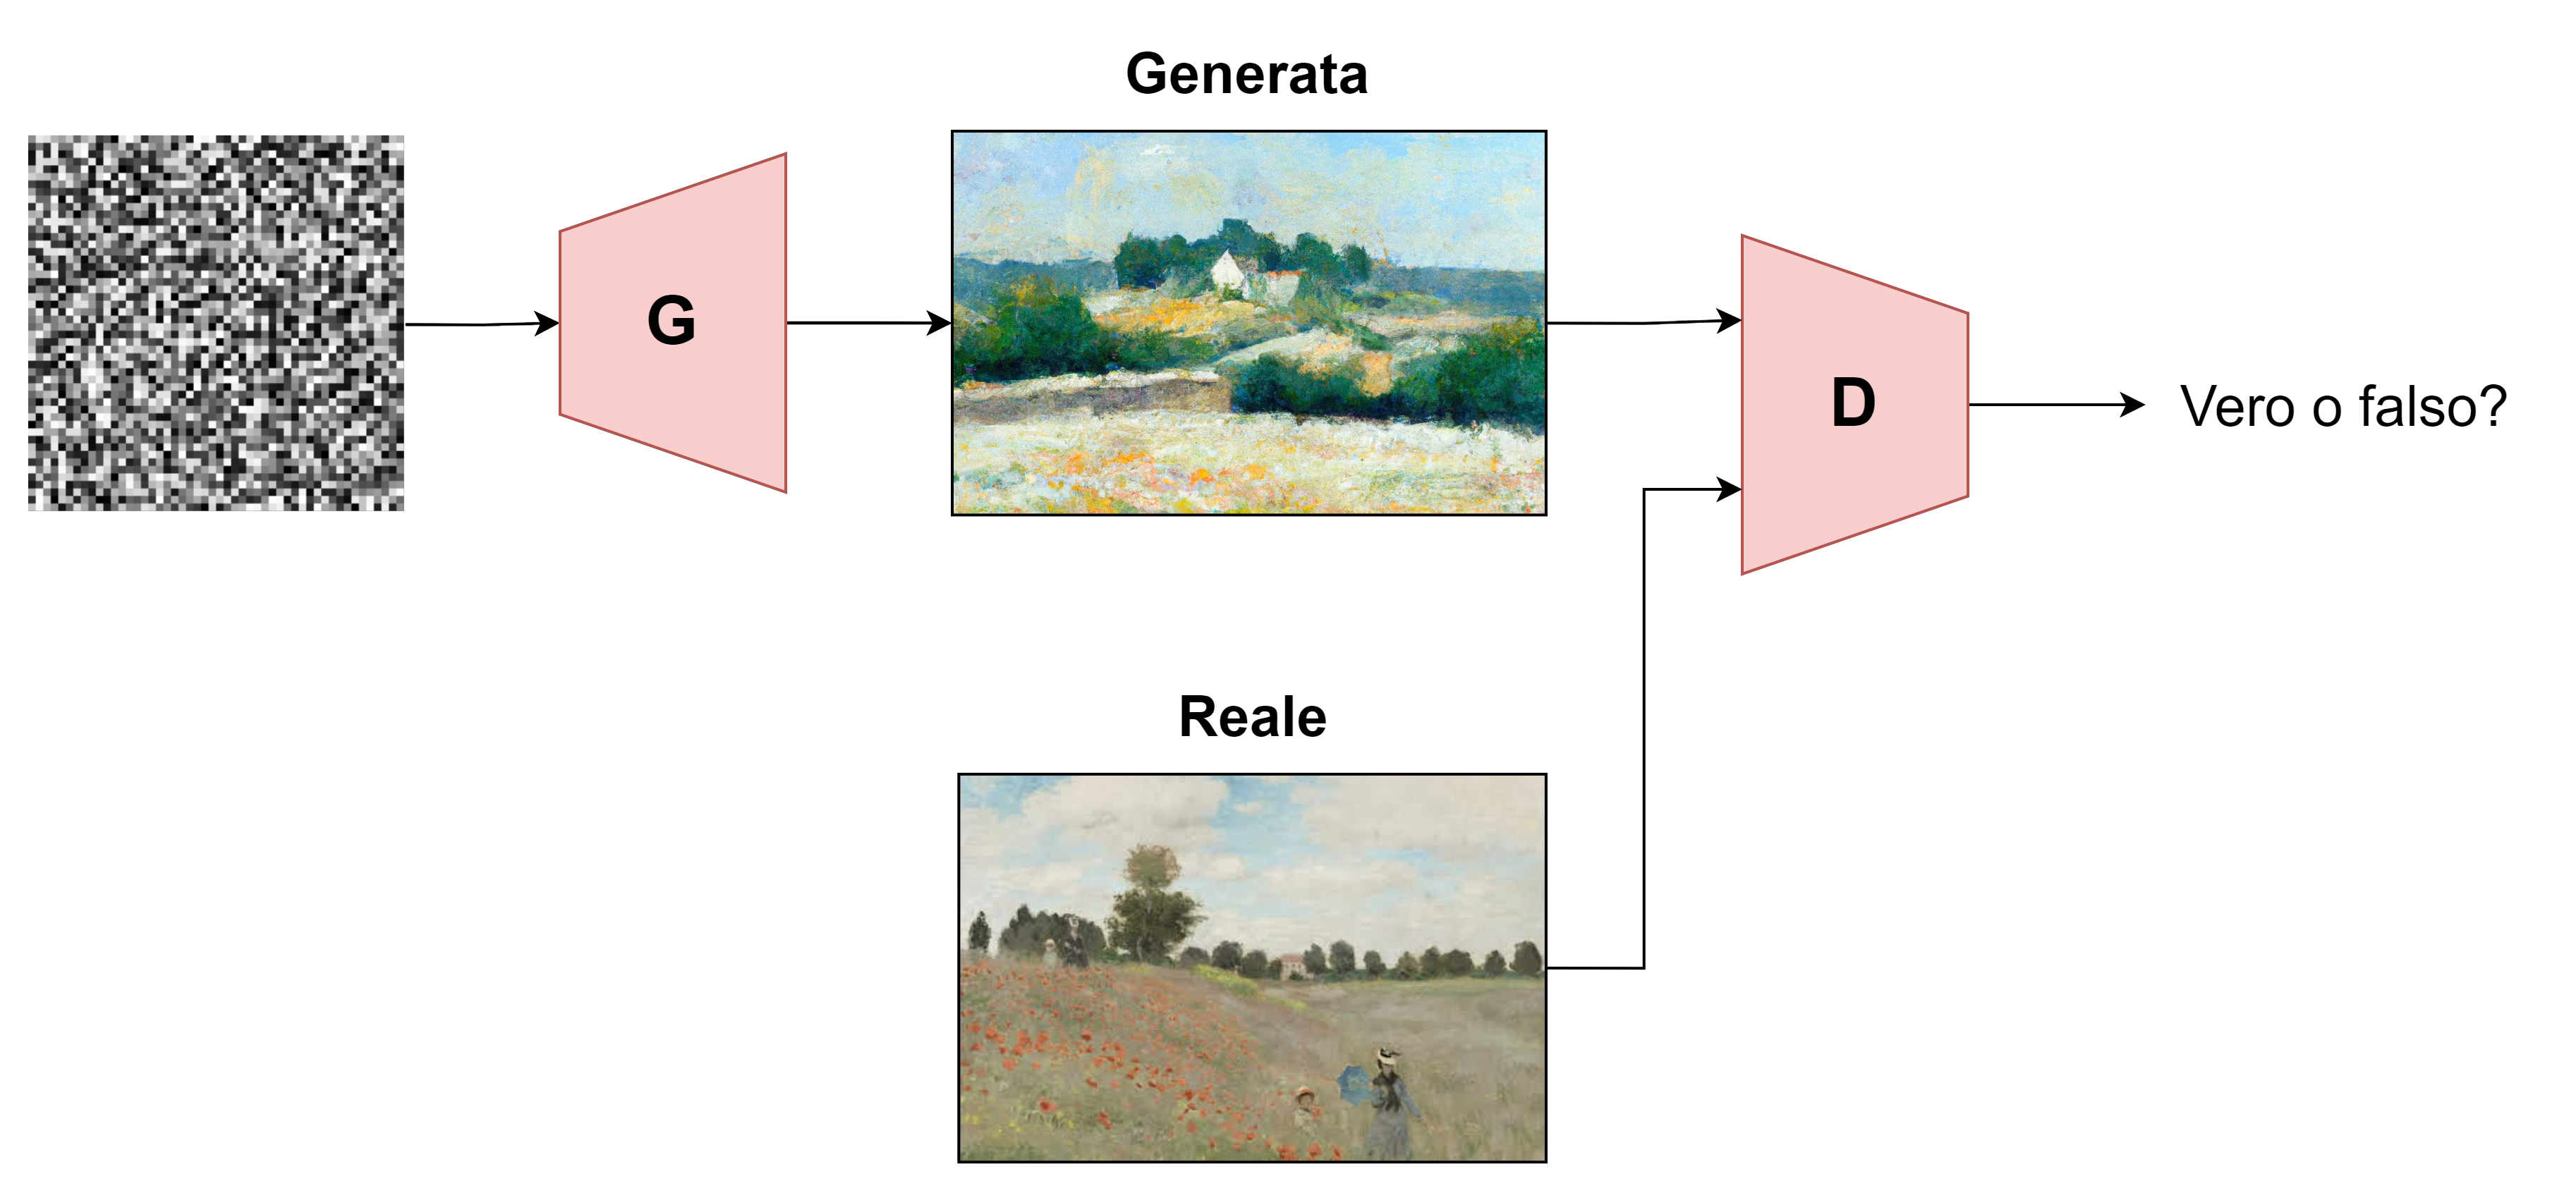
\includegraphics[width=0.7\linewidth]{figures/gans}
				\caption{GAN che genera dipinti in stile Monet.}
				\label{fig:gans}
			\end{figure}
		
		\subsection{CycleGAN}
			La \textit{image-to-image translation} è una classe di problemi nelle quali l'obiettivo è riuscire a imparare a mappare input e output di coppie di immagini. Tuttavia avere a disposizione questi dati paralleli non è sempre possibile. Basti pensare ad un convertitore di foto a dipinti, bisognerebbe dunque avere una serie di foto e dipinti corrispondenti e abbinate.
			
			Nella image-to-image translation la GAN come input, anziché rumore casuale, prende un'immagine di un certo dominio $X$ e cercherà di mapparla in un'immagine generata che abbia proprietà simili al dominio $Y$ (immagini date di rifermento al discriminatore).
			Al fine di costruire un framework che permetta di lavorare con dati non paralleli, semplificando quindi la collezione del dataset, è stata progettata la CycleGAN\cite{CycleGAN2017}.
			
			Una CycleGAN è composta da 2 GAN, una per convertire dal dominio $X$ al dominio $Y$ e una per l'inverso, e dunque da 2 generatori e 2 discriminatori.
			Nella fase di training abbiamo due cicli che si alternano: un ciclo forward e uno backward. 
			Nel ciclo forward (Fig. \ref{fig:cyclegan-forward}) viene selezionata un'immagine dal dominio $X$ e viene trasformata dal primo generatore ($G_{XY}$) in un'immagine del dominio $Y$. Questa viene testata dal discriminatore che dovrà capire se sia reale o generata. La stessa immagine viene anche trasformata nuovamente dal secondo generatore ($G_{YX}$) in un'immagine del dominio $X$ per poi essere confrontata impiegando una funzione di \textit{Cycle Consistency Loss} con l'immagine originale.

			\begin{figure}%[h]
				\centering
				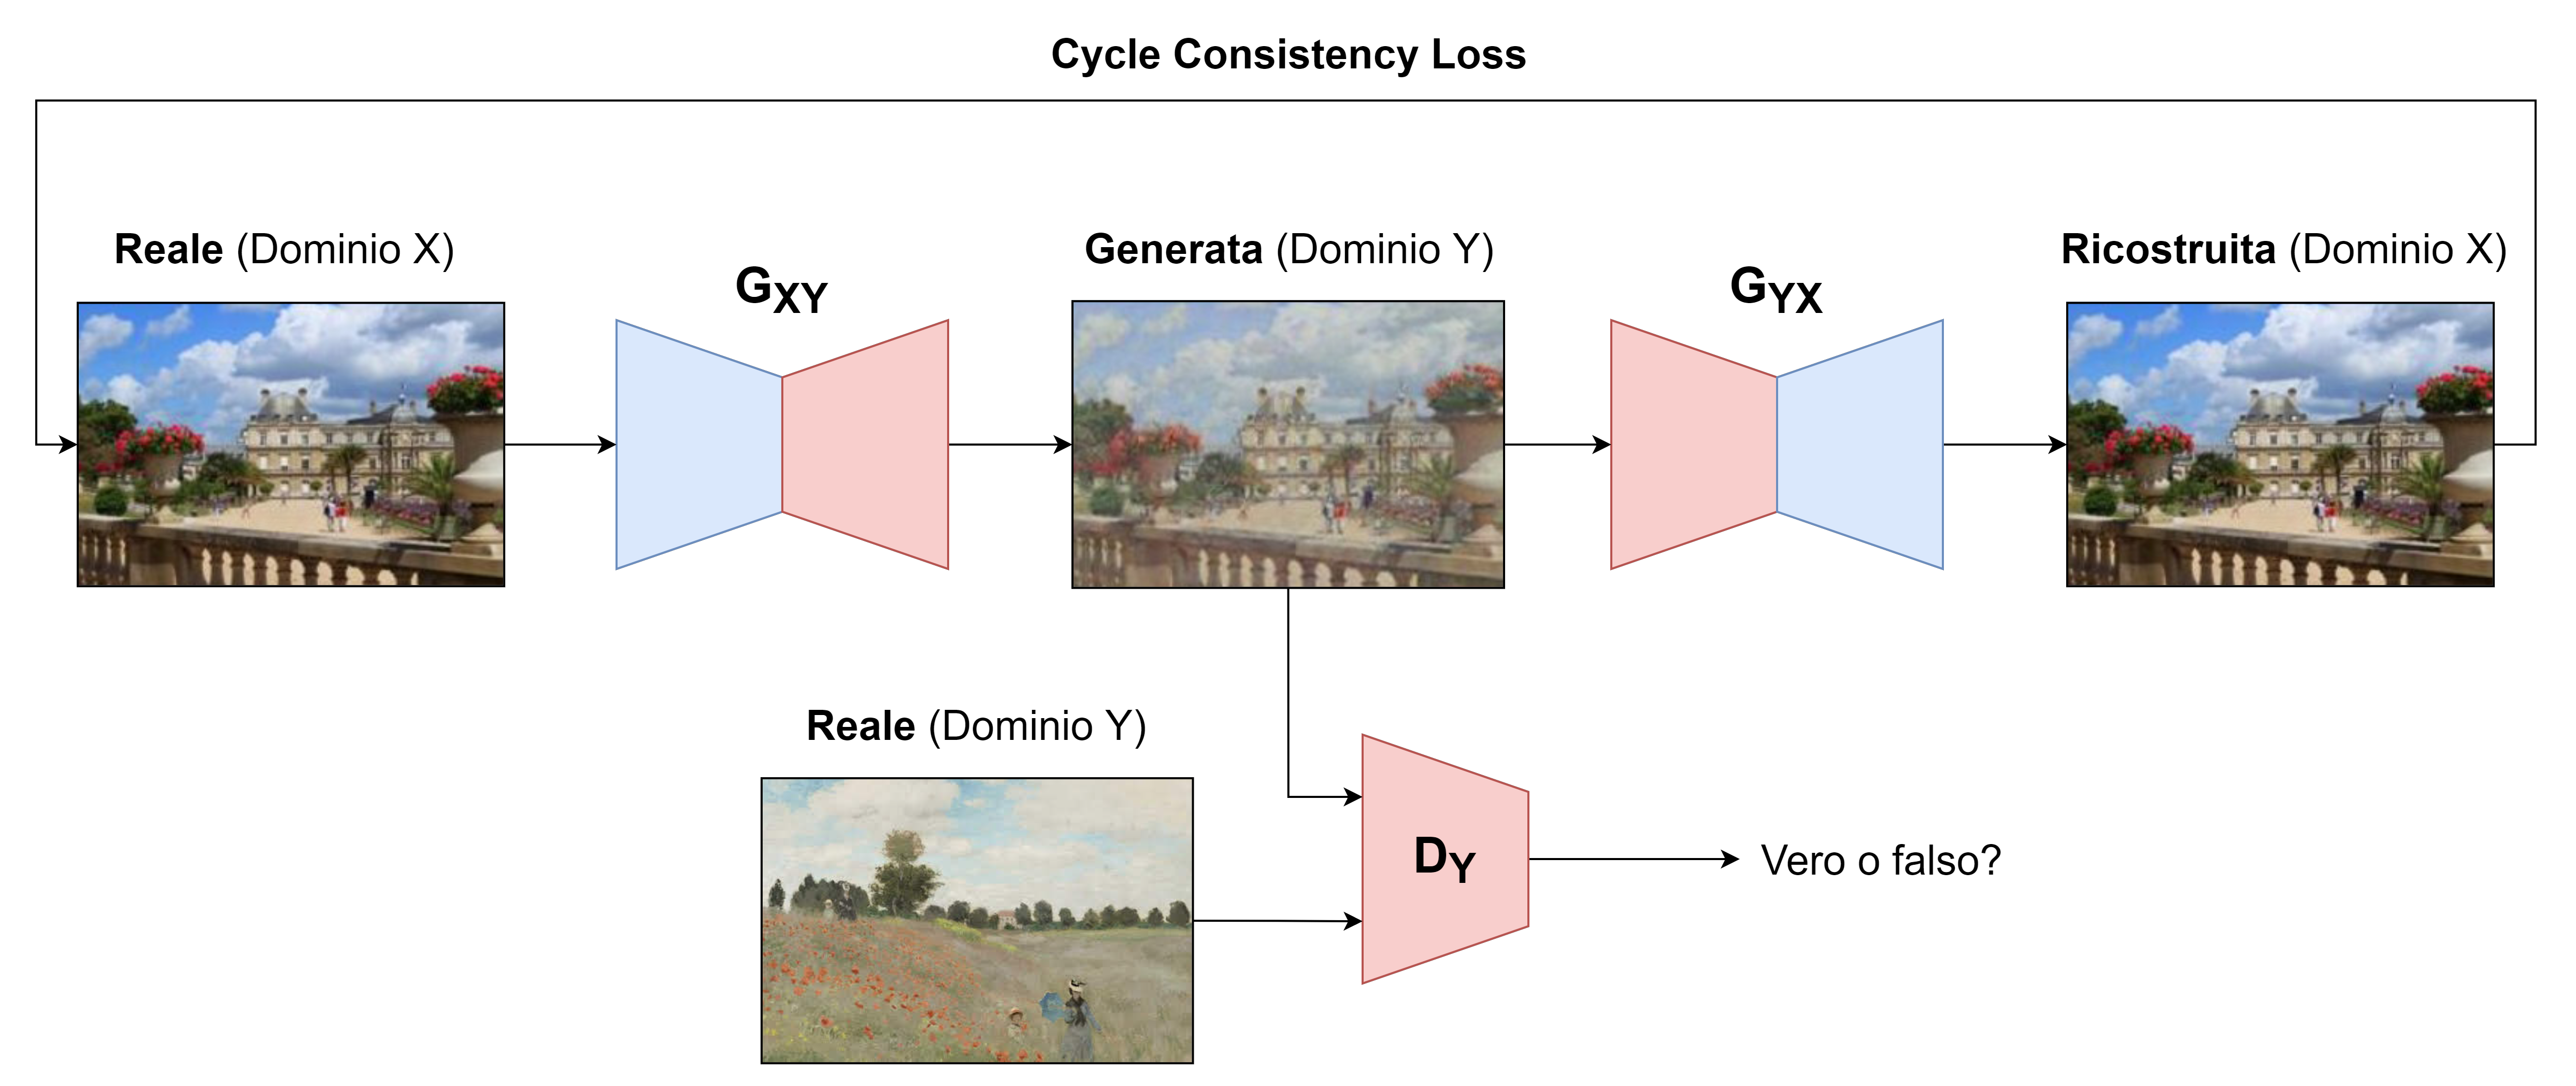
\includegraphics[width=1\linewidth]{figures/cyclegan-A2B}
				\caption{Ciclo forward della CycleGAN che trasforma foto in dipinti di Monet.}
				\label{fig:cyclegan-forward}
			\end{figure}
			
			Nel ciclo backward avviene la stessa operazione del ciclo forward ma partendo dal dominio $Y$ e usando gli opportuni generatori e discrimantori come illustrato in Fig. \ref{fig:cyclegan-backward}.
			\begin{figure}%[h]
			\centering
			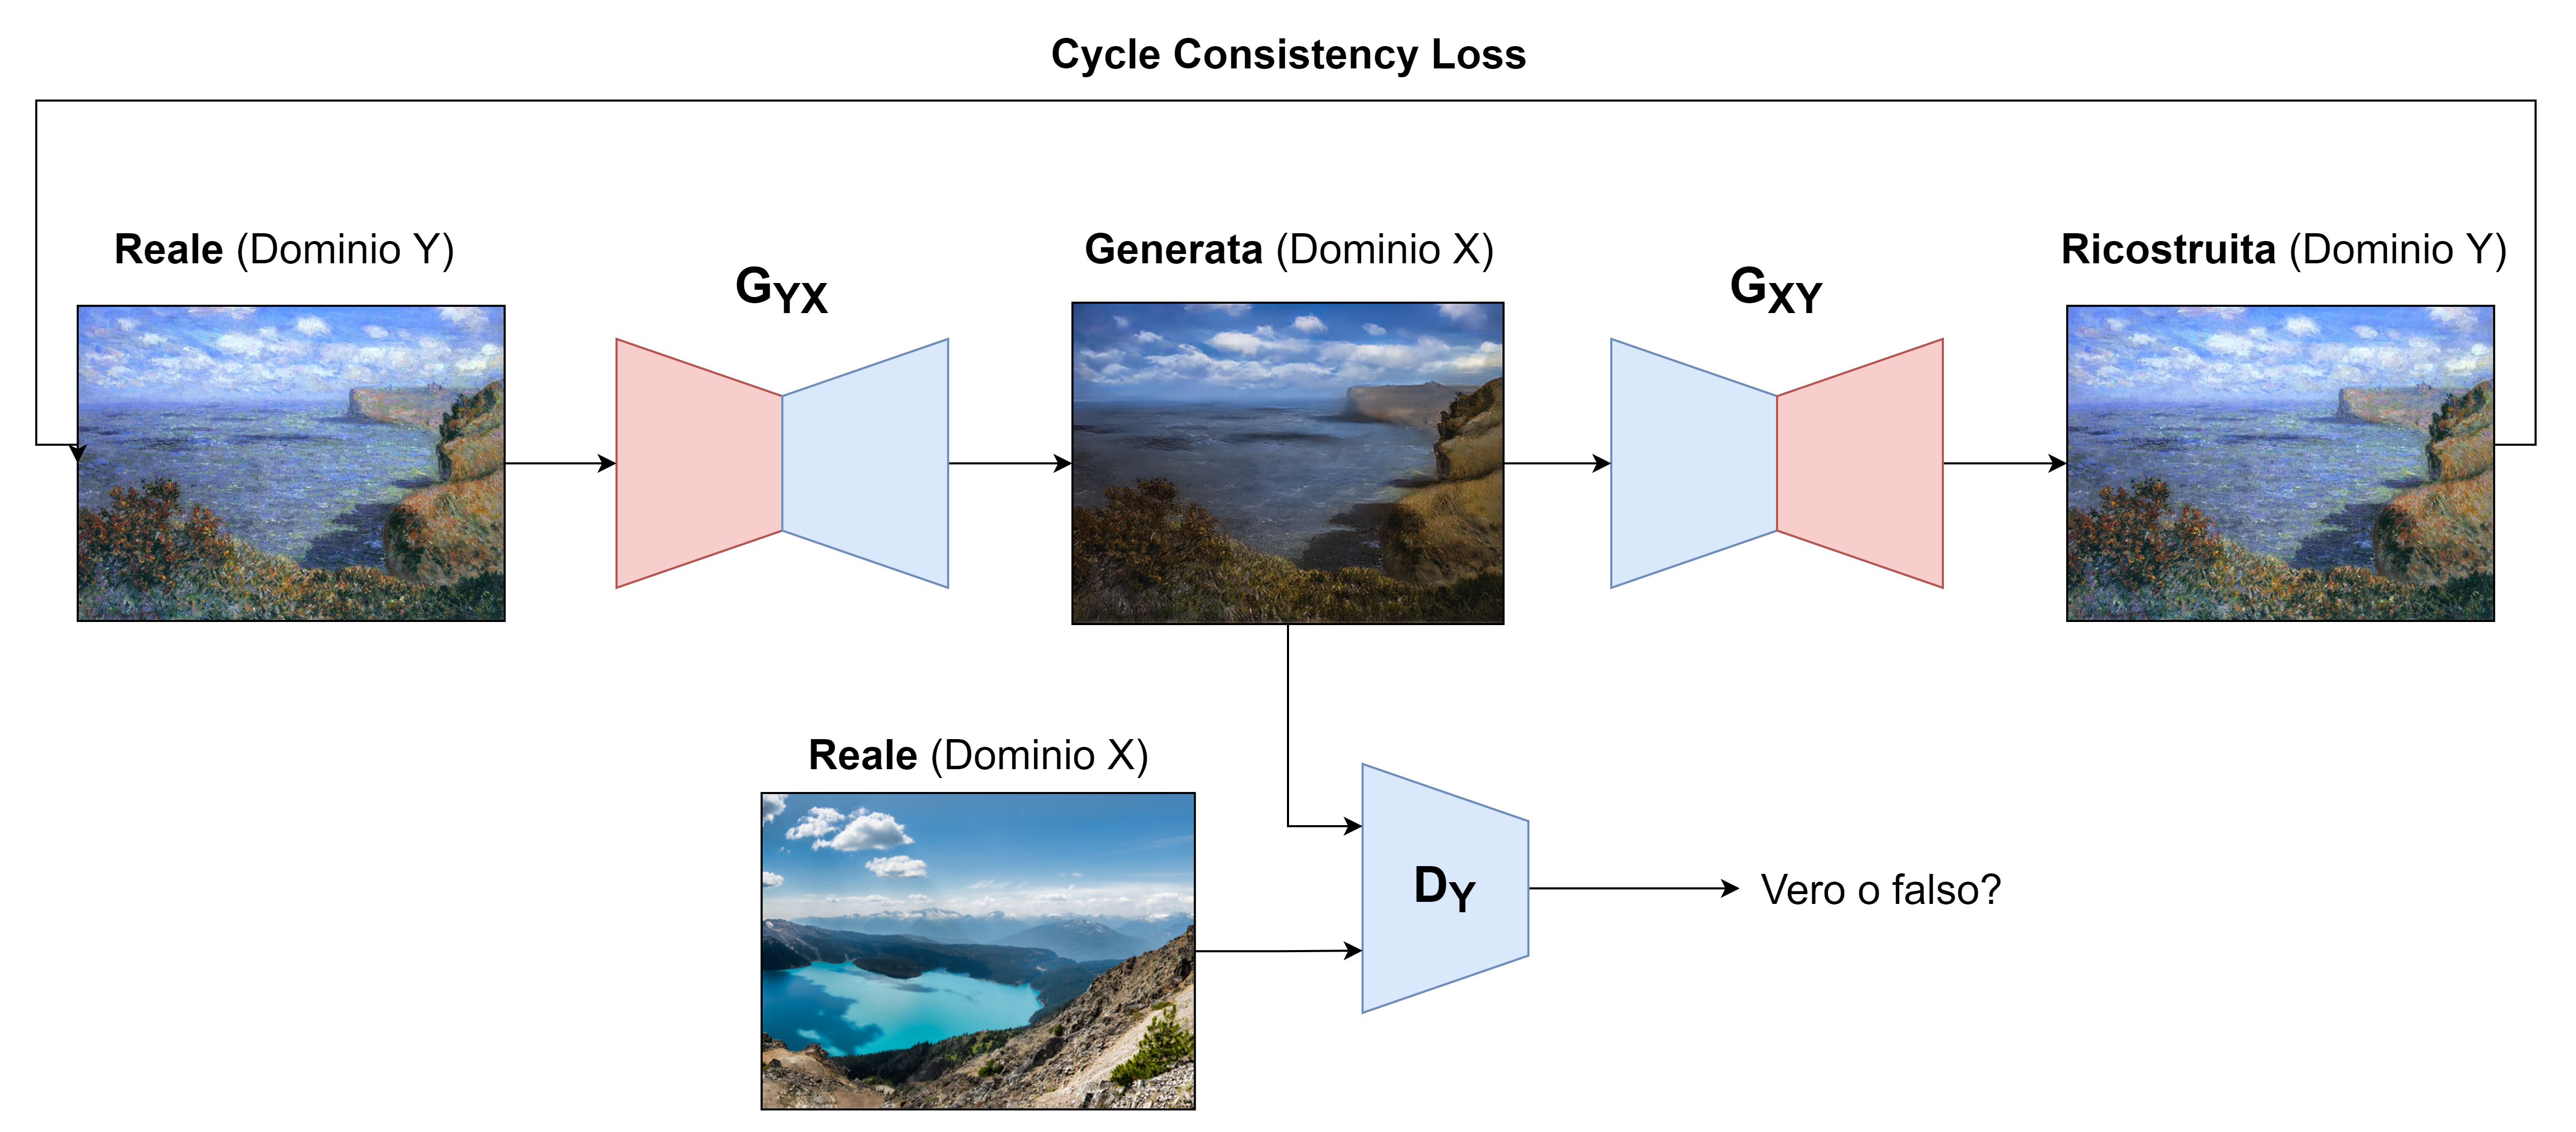
\includegraphics[width=1\linewidth]{figures/cyclegan-B2A}
			\caption{Ciclo backward della CycleGAN che trasforma foto in dipinti di Monet.}
			\label{fig:cyclegan-backward}
			\end{figure}
	
		\subsection{MelGAN}
		Elaborare segnali audio è un processo complesso che richiede spesso il passaggio a rappresentazioni intermedie che possono portare artefatti e comprometterne i risultati.
		Nel 2019 viene proposto da Kumar un vocoder neurale per spettrogrammi mel basato su reti generative avversarie: MelGAN\cite{melgan}.
		L'architettura è una fully convolutional network che prende in input spettrogrammi mel e fornisce come output l'audio corrispondente.
		
		\subsection{CycleGAN-VCs}
			Di seguito vengono descritte le architetture delle CycleGAN-VCs per poter vedere quali sono i passi che hanno portato ad ottenere la MaskCycleGAN-VC, ovvero la rete impiegata in questo lavoro.
			
			\paragraph{CycleGAN-VC}
			Nel 2017 Kaneko e Kameoka propongono un metodo per la voice conversion che permette di imparare a mappare una voce source in una target senza bisogno di dati paralleli. Il metodo, chiamato CycleGAN-VC, si basa sull'architettura di una CycleGAN a cui vengono applicate due modifiche: l'impiego di gated CNN e l'impiego di una identity-mapping loss (Fig. \ref{fig:cyclegan-vc})\cite{CycleGAN-VC}.
			
			L'introduzione di gated CNN all'interno della rete permette di conservare la struttura gerarchica della voce mantenendo un costo computazionale piuttosto basso mentre l'impiego di una funzione di identità (\ref{eq:identity}) ha lo scopo di mantenere il contenuto linguistico intatto.
			\begin{equation}
				\mathcal{L}_{id}(G_{XY}, G_{YX}) = \mathbb{E}_{y \sim P_{Data}(y)}[||G_{XY}(y) - y||_1] \\
				+ \mathbb{E}_{x \sim P_{Data}(x)}[||G_{YX}(x) - x||_1]
			\label{eq:identity}
			\end{equation}
			
			\begin{figure}[h]
				\centering
				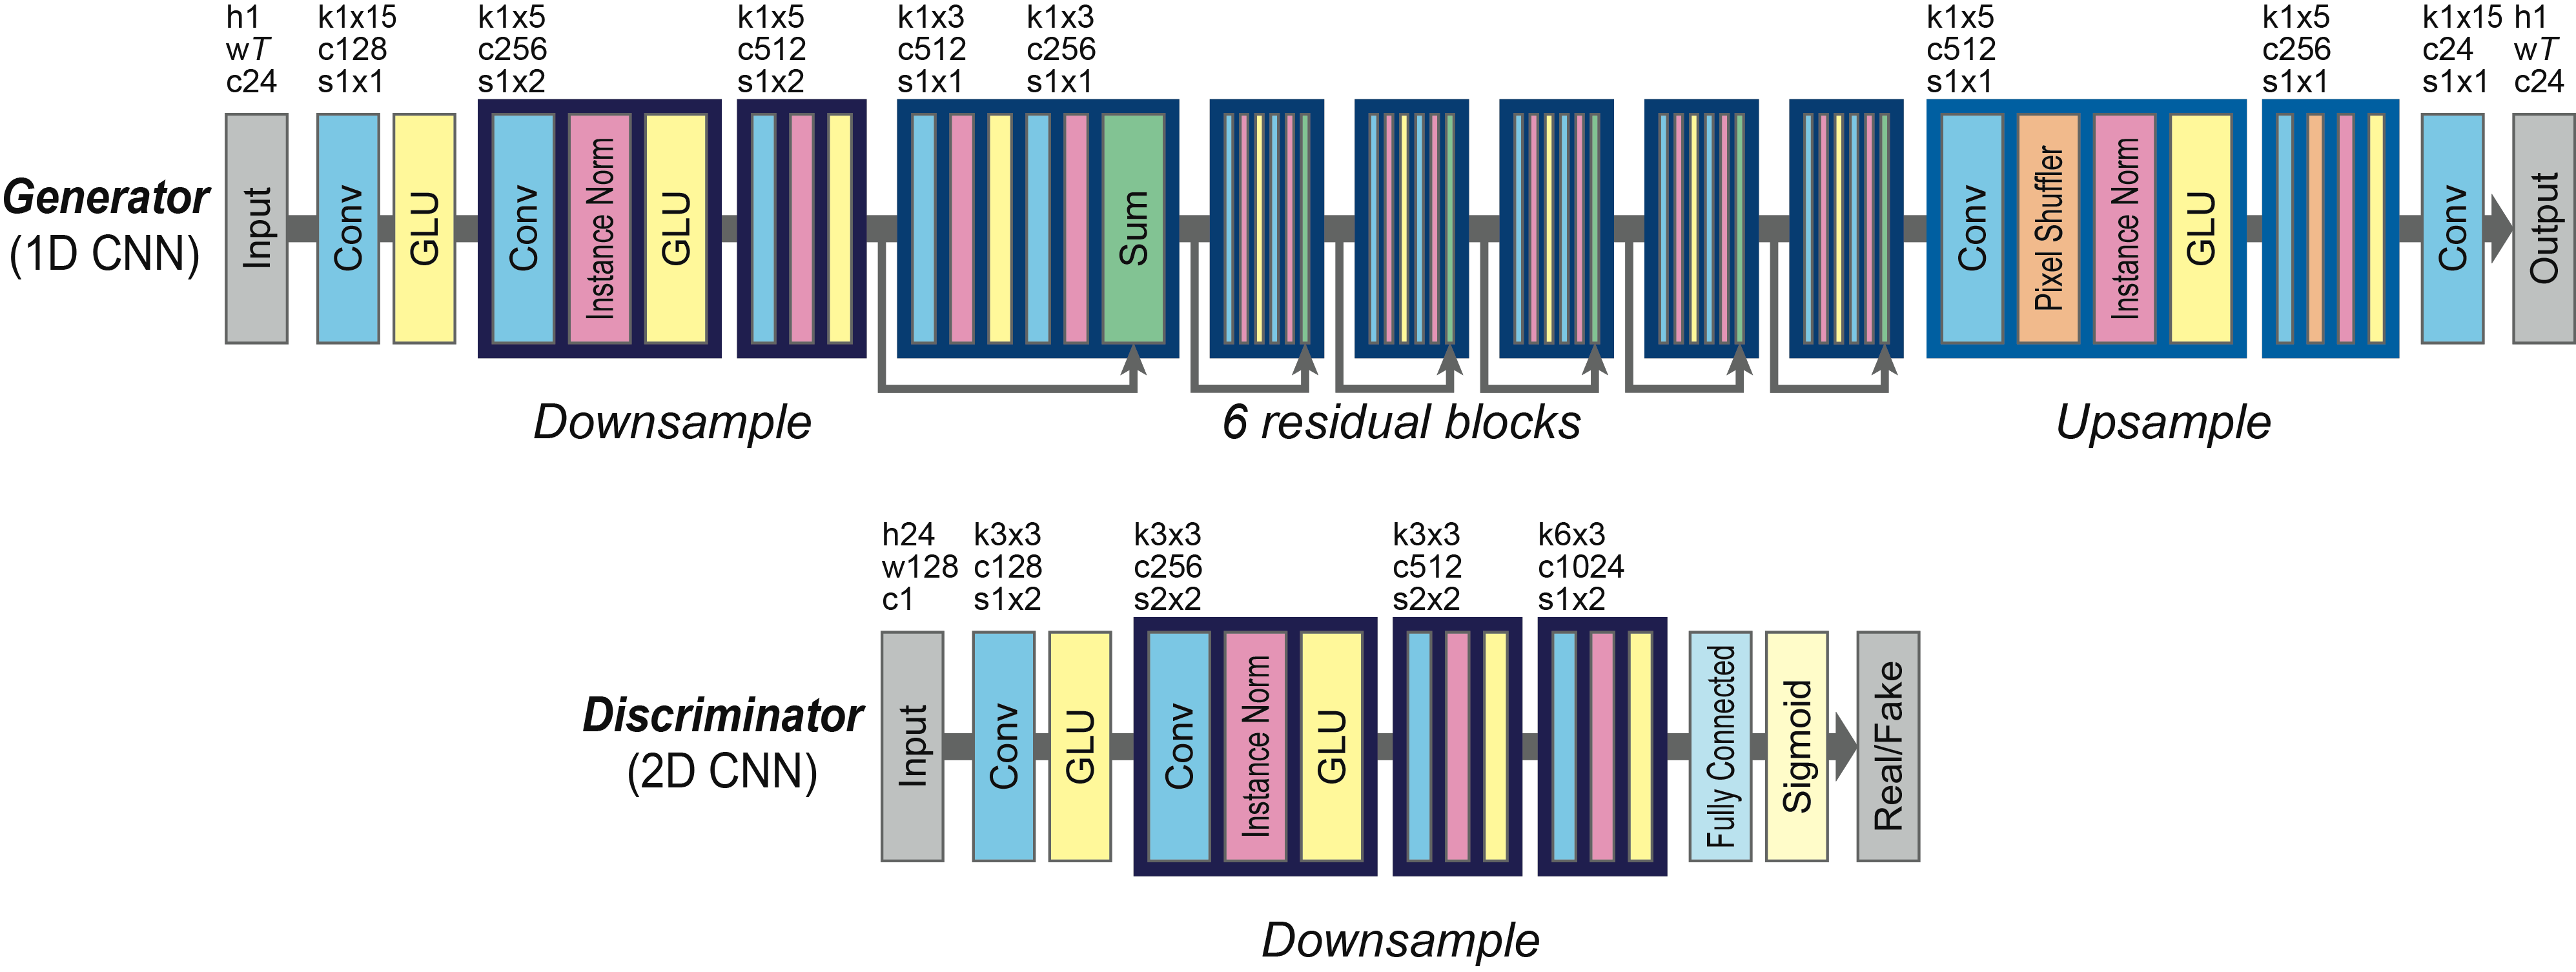
\includegraphics[width=1\linewidth]{figures/CycleGAN-VC}
				\caption{Architettura di CycleGAN-VC. Fonte \cite{CycleGAN-VC}.}
				\label{fig:cyclegan-vc}
			\end{figure}
		
			Il modello utilizza coefficienti mel cepstrum, frequenza fondamentale logaritmica e aperiodicità come feature per la conversione.
			I risultati ottenuti sono di particolare interesse in quanto simili a procedure con impiego di dati paralleli senza necessitare di ulteriori dati o dell'allineamento temporale di questi.
		
			\paragraph{CycleGAN-VC2}
			Successivamente, nel 2019 viene proposta una versione migliorata, chiamata CycleGAN-VC2 (Fig. \ref{fig:cyclegan-vc2}), che incorpora tre principali cambiamenti: introduzione di una seconda adversarial loss (\ref{eq:second-loss}), generatore migliorato (2-1-2D CNN) e discriminatore migliorato (PatchGAN)\cite{CycleGAN-VC2}. 
			\begin{equation}
				\mathcal{L}_{adv2}^{X \rightarrow Y \rightarrow X} = \mathbb{E}_{x \sim P_X}[log D'_X(x)] + \mathbb{E}_{x \sim P_X}[log(1-D'_X(G_{YX}(G_{XY}(x))))]
				\label{eq:second-loss}
			\end{equation}
			
			\begin{figure}[h]
				\centering
				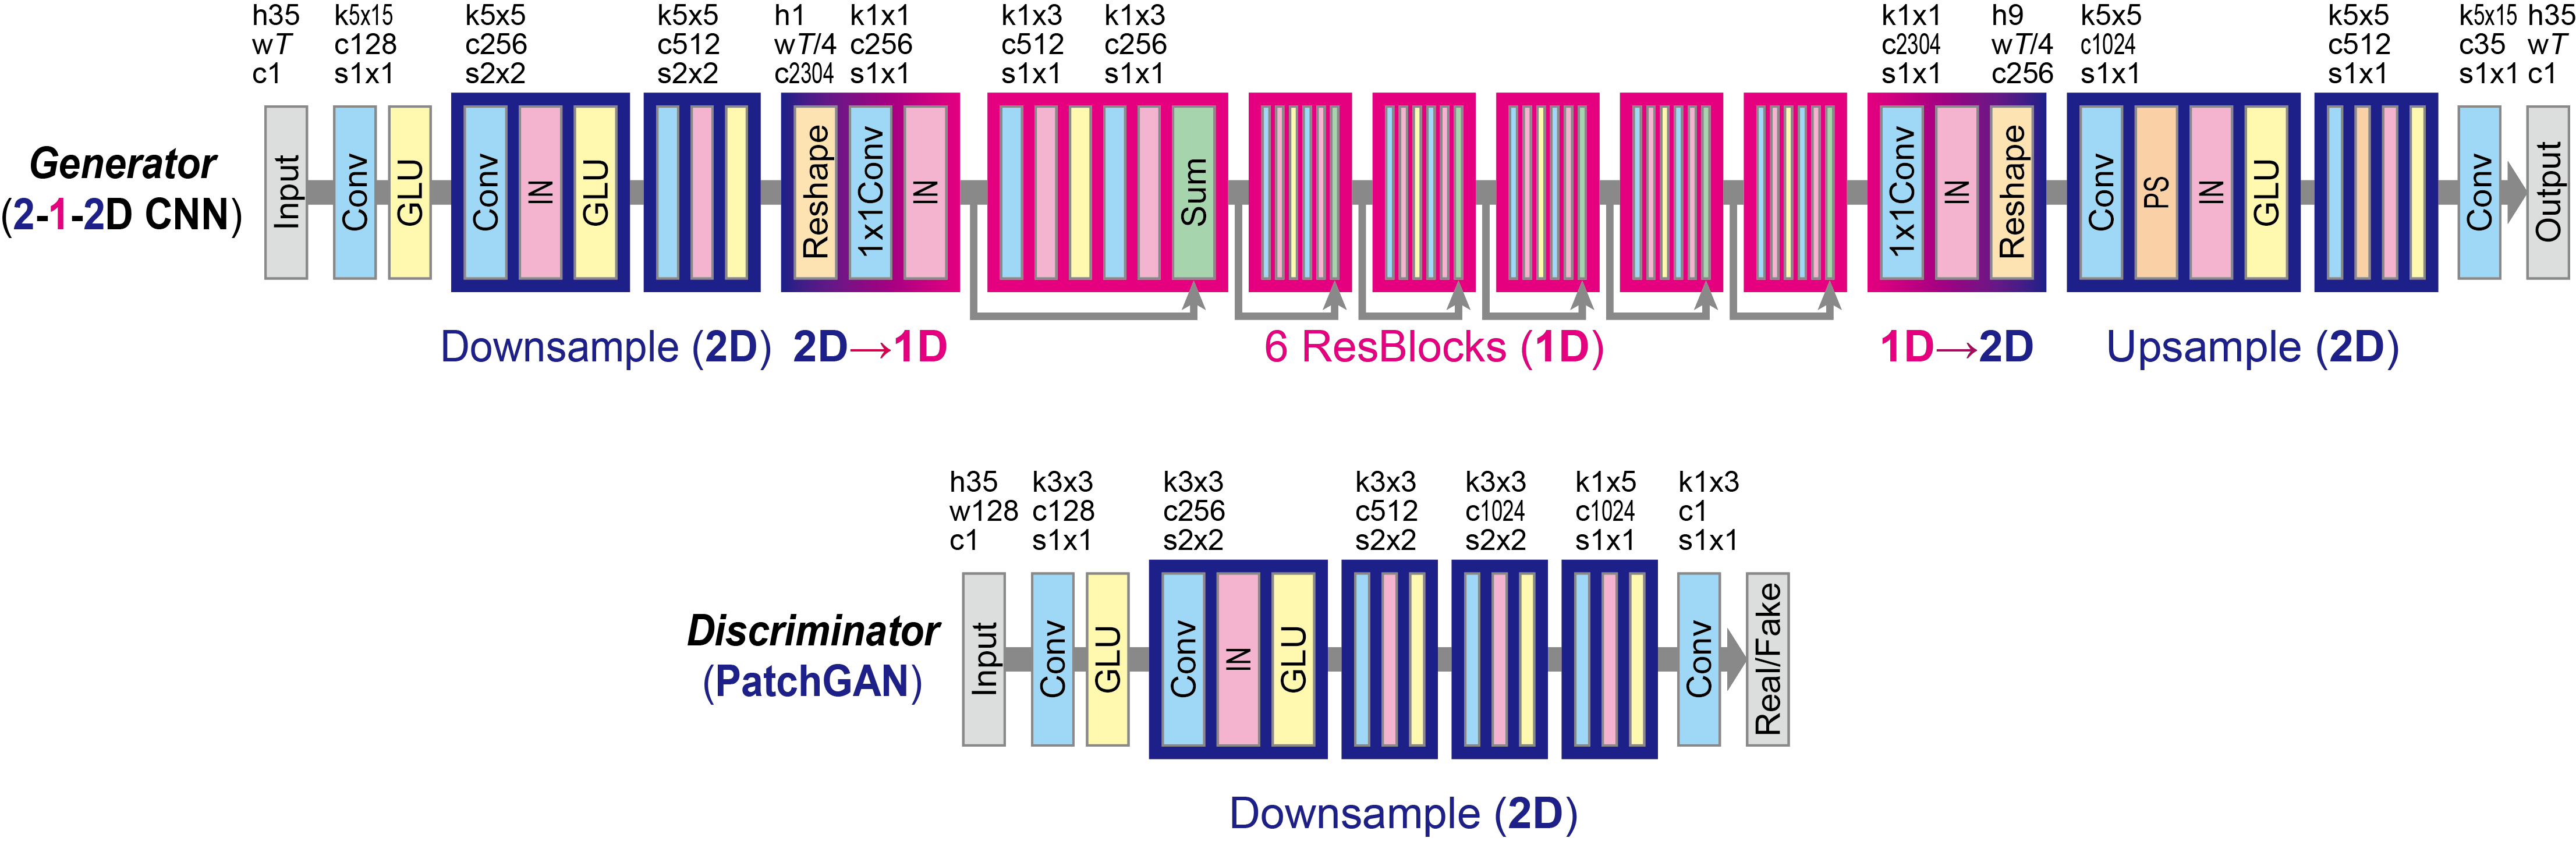
\includegraphics[width=1\linewidth]{figures/CycleGAN-VC2}
				\caption{Architettura di CycleGAN-VC2. Fonte \cite{CycleGAN-VC2}.}
				\label{fig:cyclegan-vc2}
			\end{figure}
			
			\paragraph{CycleGAN-VC3}
			Gli ottimi risultati ottenuti dalle CycleGAN-VCs hanno portato all'impiego di queste come metodi di benchmark per altri studi. Questo però ha evidenziato la necessità di confrontare i risultati sotto forma di spettrogrammi mel. Tuttavia impiegando spettrogrammi mel, al posto di coefficienti mel cepstrum, direttamente come input di queste reti, si producono risultati scarsi dovuti alla compromissione della struttura temporale del segnale.
			
			Al fine di ovviare a questo problema viene proposta CycleGAN-VC3 (Fig. \ref{fig:cyclegan-vc3}) che incorpora una normalizzazione adattiva sul dominio tempo-frequenza (TFAN)\cite{CycleGAN-VC3}.
			\begin{figure}[h]
				\centering
				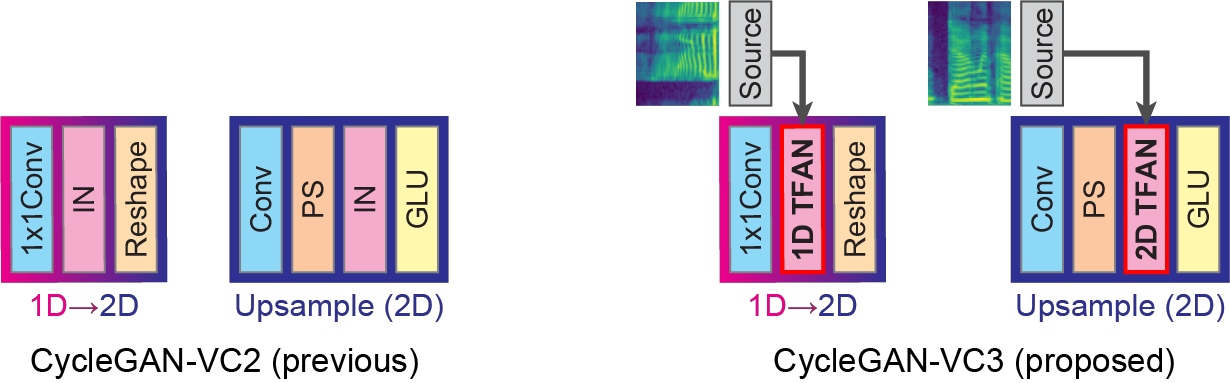
\includegraphics[width=0.8\linewidth]{figures/CycleGAN-VC3}
				\caption{Comparazione di CycleGAN-VC3 rispetto a CycleGAN-VC2. In CycleGAN-VC3 viene incorporato TFAN nel generatore di CycleGAN-VC2. In particolare viene rimpiazzato nel blocco 1D$\rightarrow$2D e nel blocco Upsample. Fonte \cite{CycleGAN-VC3}.}
				\label{fig:cyclegan-vc3}
			\end{figure}
		
			\paragraph{MaskCycleGAN-VC}
			La MaskCycleGAN-VC (Fig. \ref{fig:maskcyclegan-vc}) è una variante della CycleGAN-VC2 che, come la CycleGAN-VC3, impiega spettrogrammi mel al posto di coefficienti mel cepstrum \cite{MaskCyclegan-VC}.
			
			Tra le modifiche principali rispetto alla precedente CycleGAN-VC3, questa architettura non impiega il modulo aggiuntivo TFAN, che comportava un incremento del numero di parametri da imparare, ma sfrutta invece una tecnica di \textit{filling in frames} (FIF).
			Con tale tecnica vengono applicate maschere temporali durante la fase di addestramento, che hanno lo scopo di far apprendere al modello come riempire il frame mancante in base al contesto.
			
			Si procede con la descrizione del funzionamento dell'architettura.
			Dato uno spettrogramma mel $x$, viene prima creata una maschera temporale $m$ e viene moltiplicata ad esso. Si ottiene quindi un nuovo spettrogramma mel $\hat{x}$ a cui è stati rimossi dei frame:
			\begin{equation}
				\hat{x}=x \cdot m
			\end{equation}
			Si procede a passare al convertitore $\hat{x}$ e la sua maschera $m$, ottenendo la sua conversione $y'$:
			\begin{equation}
				y' = G_{XY}^{mask}(concat(\hat{x}, m))
			\end{equation}
			Passando la maschera esplicitamente, si permette al convertitore di sapere dove andare a generare informazioni mancanti.
			Viene calcolata la adversarial loss per assicurarsi che $y'$ sia nell'insieme target $Y$ e viene inoltre convertita nuovamente nel dominio $X$. Si ricostruisce dunque $x''$ applicando una maschera fittizia $m'$ che non rimuoverà alcun frame (una matrice di soli uno):
			\begin{equation}
				x'' = G_{YX}^{mask}(concat(y', m'))
			\end{equation}
			Si applica quindi la cycle-consistency loss per lo spettrogramma mel ricostruito e viene calcolata la seconda adversarial loss (\ref{eq:second-loss}).
			\begin{equation}
				\mathcal{L}_{mcyc}^{X \rightarrow Y \rightarrow X} = \mathbb{E}_{x \sim P_X,m \sim P_M}[||x''-x||_1]
			\end{equation}
			
			\begin{figure}[h]
				\centering
				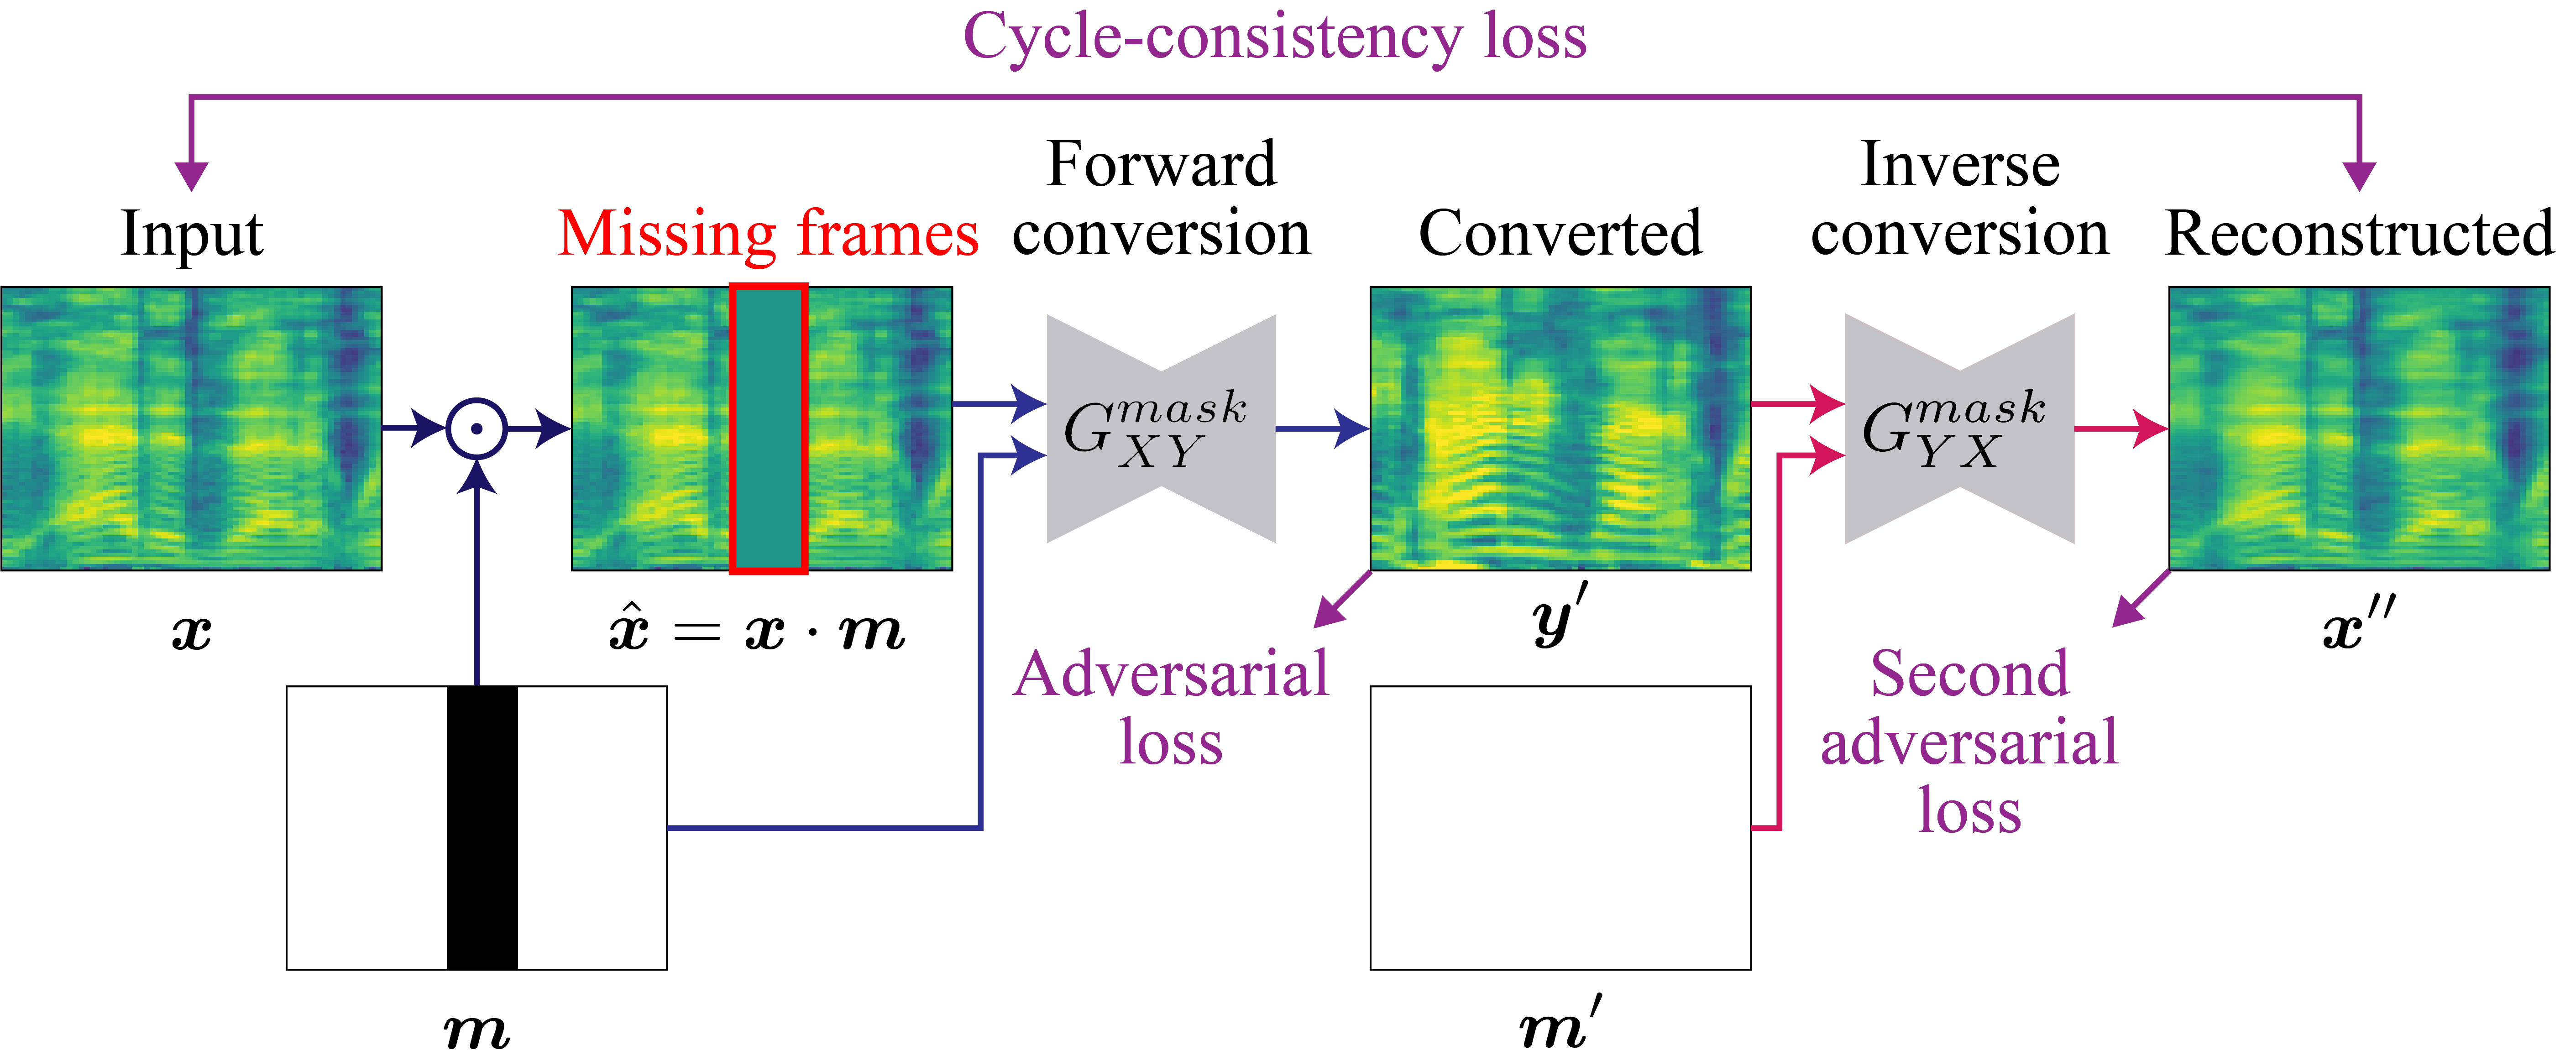
\includegraphics[width=1\linewidth]{figures/MaskCycleGAN-VC}
				\caption{Ciclo forward dell'architettura MaskCycleGAN-VC. Fonte \cite{MaskCyclegan-VC}.}
				\label{fig:maskcyclegan-vc}
			\end{figure}
			
			
		
	\chapter{Architettura proposta}
	\label{chap:architettura-proposta}
		In questo capitolo sarà descritta l'architettura del framework sviluppato per la conversione di voci a spettro ridotto mediante l'utilizzo di vocoded speech e di sine-wave speech.
		
		\section{Metodo}
		L'idea alla base di questo framework è la conversione di voci tra due speaker differenti che andremo a chiamare $X$ (sorgente) e $Y$ (target).
		
		L'innovazione principale del framework proposto è la riduzione dello spettro sonoro, processo attraverso il quale si riducono le caratteristiche acustiche dello speaker sorgente $X$.
		
		Andremo a presentare due moduli per questo scopo: un modulo di riduzione a sine-wave speech (SWS) e uno di riduzione a vocoded speech.
	
		\begin{figure}[h]
			\centering
			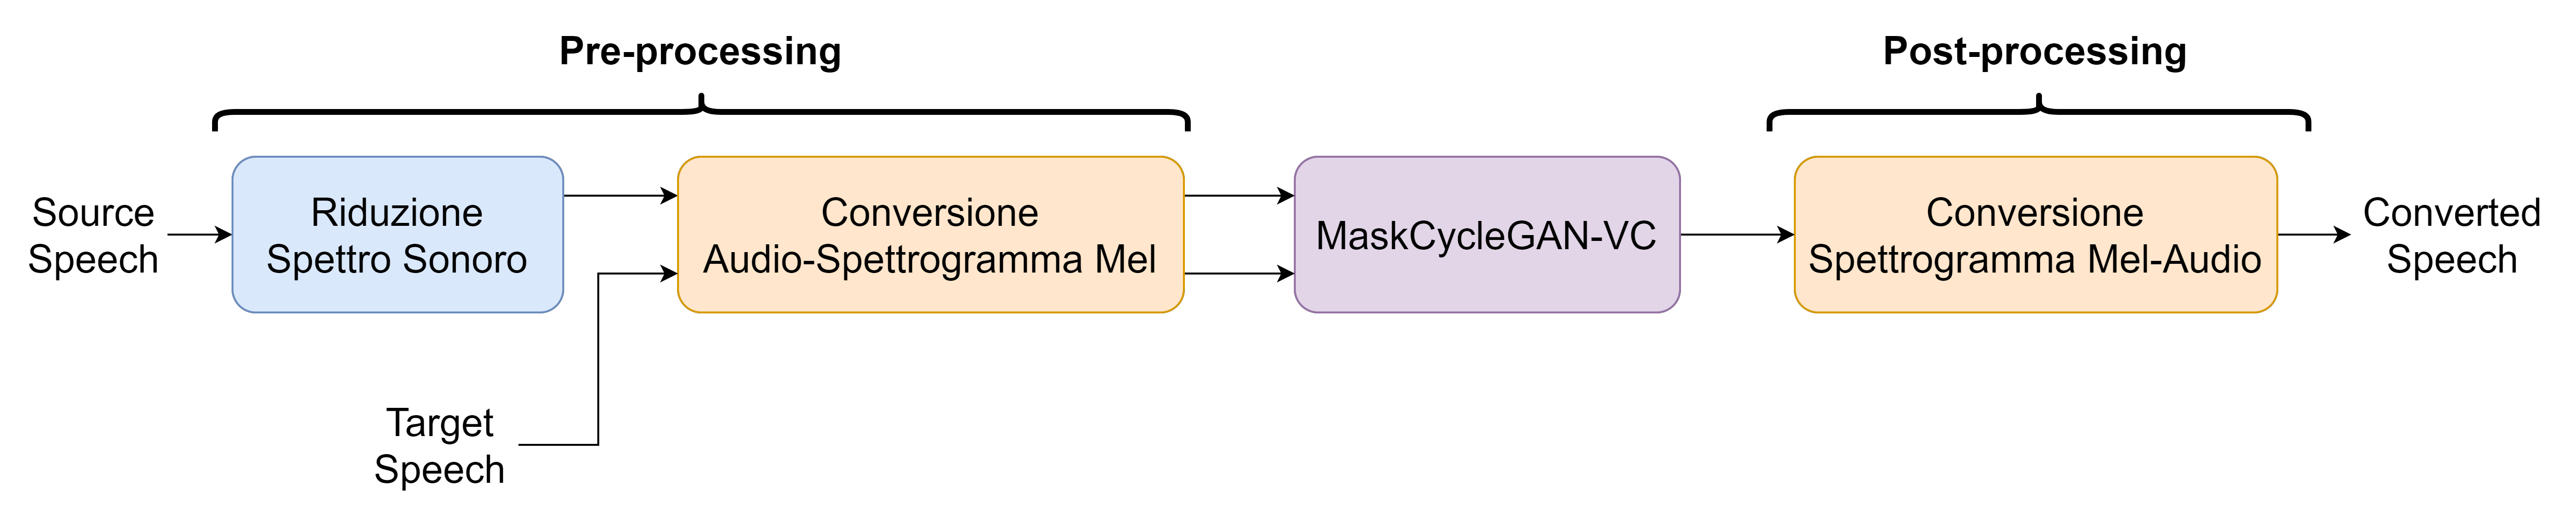
\includegraphics[width=1\linewidth]{figures/MaskCycleGAN-SWS-VC-pipeline}
			\caption{Pipeline dell'architettura proposta.}
			\label{fig:maskcyclegan-sws-vc-pipeline}
		\end{figure}		
		
		\section{Modulo di riduzione dello spettro sonoro}
		\label{sec:proposta-riduzione}
			I seguenti moduli sono parte della fase di pre-processamento dell'audio (Fig. \ref{fig:maskcyclegan-sws-vc-pipeline} e \ref{fig:modulo-riduzione-spettro-sonoro}).			
		
			\subsection{Modulo di riduzione a vocoded speech}
			Il metodo implementato per generare il vocoded speech si basa su Linear Predictive Coding (LPC), impiegando l'algoritmo di Burg\cite{burg-algorithm}.
			Si descrive di seguito la procedura applicata:
			\begin{itemize}
				\item L'audio originale viene ricampionato a 8 kHz. In questo modo la frequenza di Nyquist, che per definizione si attesta a $ \frac{1}{2} f_{s} $, sarà di 4 kHz ovvero sarà possibile rappresentare senza distorsioni suoni fino a tale frequenza. Tale range di frequenze viene usato come banda standard per la voce in comunicazioni telefoniche. 
				\item Vengono estratte finestre di 200 sample dell'audio.
				\item Per ogni finestra vengono calcolati i coefficienti del filtro lineare di ordine 8.
				\item Viene generato un segnale carrier della durata di 200 sample (es. buzz a 500 Hz oppure noise).
				\item Viene applicato un filtro lineare del resiudo LPC al carrier in modo da ricostruire il segnale vocale su di esso.
				\item Viene calcolata la magnitudine della finestra e viene adattato il segnale generato ad essa.
				\item L'audio viene ricostruito e ricampionato alla frequenza originale.
			\end{itemize}
		
			\subsection{Modulo di riduzione a SWS}
			Al fine di trasformare degli audio in forma sine-wave speech abbiamo la necessità di trovare le formanti e rimpiazzarle con delle onde sinusoidali pure. Il metodo implementato si basa sulla stima delle posizioni delle formanti data dalla Linear Predictive Coding (LPC)\cite{formants-from-lpc}, utilizzando l'algoritmo di Burg\cite{burg-algorithm}.
			Si descrive di seguito la procedura applicata:
			\begin{itemize}
				\item L'audio originale viene ricampionato a 8 kHz.
				\item Vengono estratte finestre di 200 sample dell'audio.
				\item Per ogni finestra vengono calcolati i coefficienti del filtro lineare di ordine 12 e si ottengono le frequenze delle formanti. La scelta dell'ordine deriva dalla seguente formula $ o = 2 \cdot n_{f} + 2 $, dove $ n_{f} $ rappresenta il numero delle formanti da trovare.
				\item Viene calcolata la magnitudine della finestra.
				\item Vengono interpolate le formanti al fine di creare 3 segnali sinusoidali mobili.
				\item Si ricostruisce l'audio alla frequenza di campionamento originale con sinusoidi alle frequenze delle formanti.
			\end{itemize}
			\begin{figure}
				\centering
				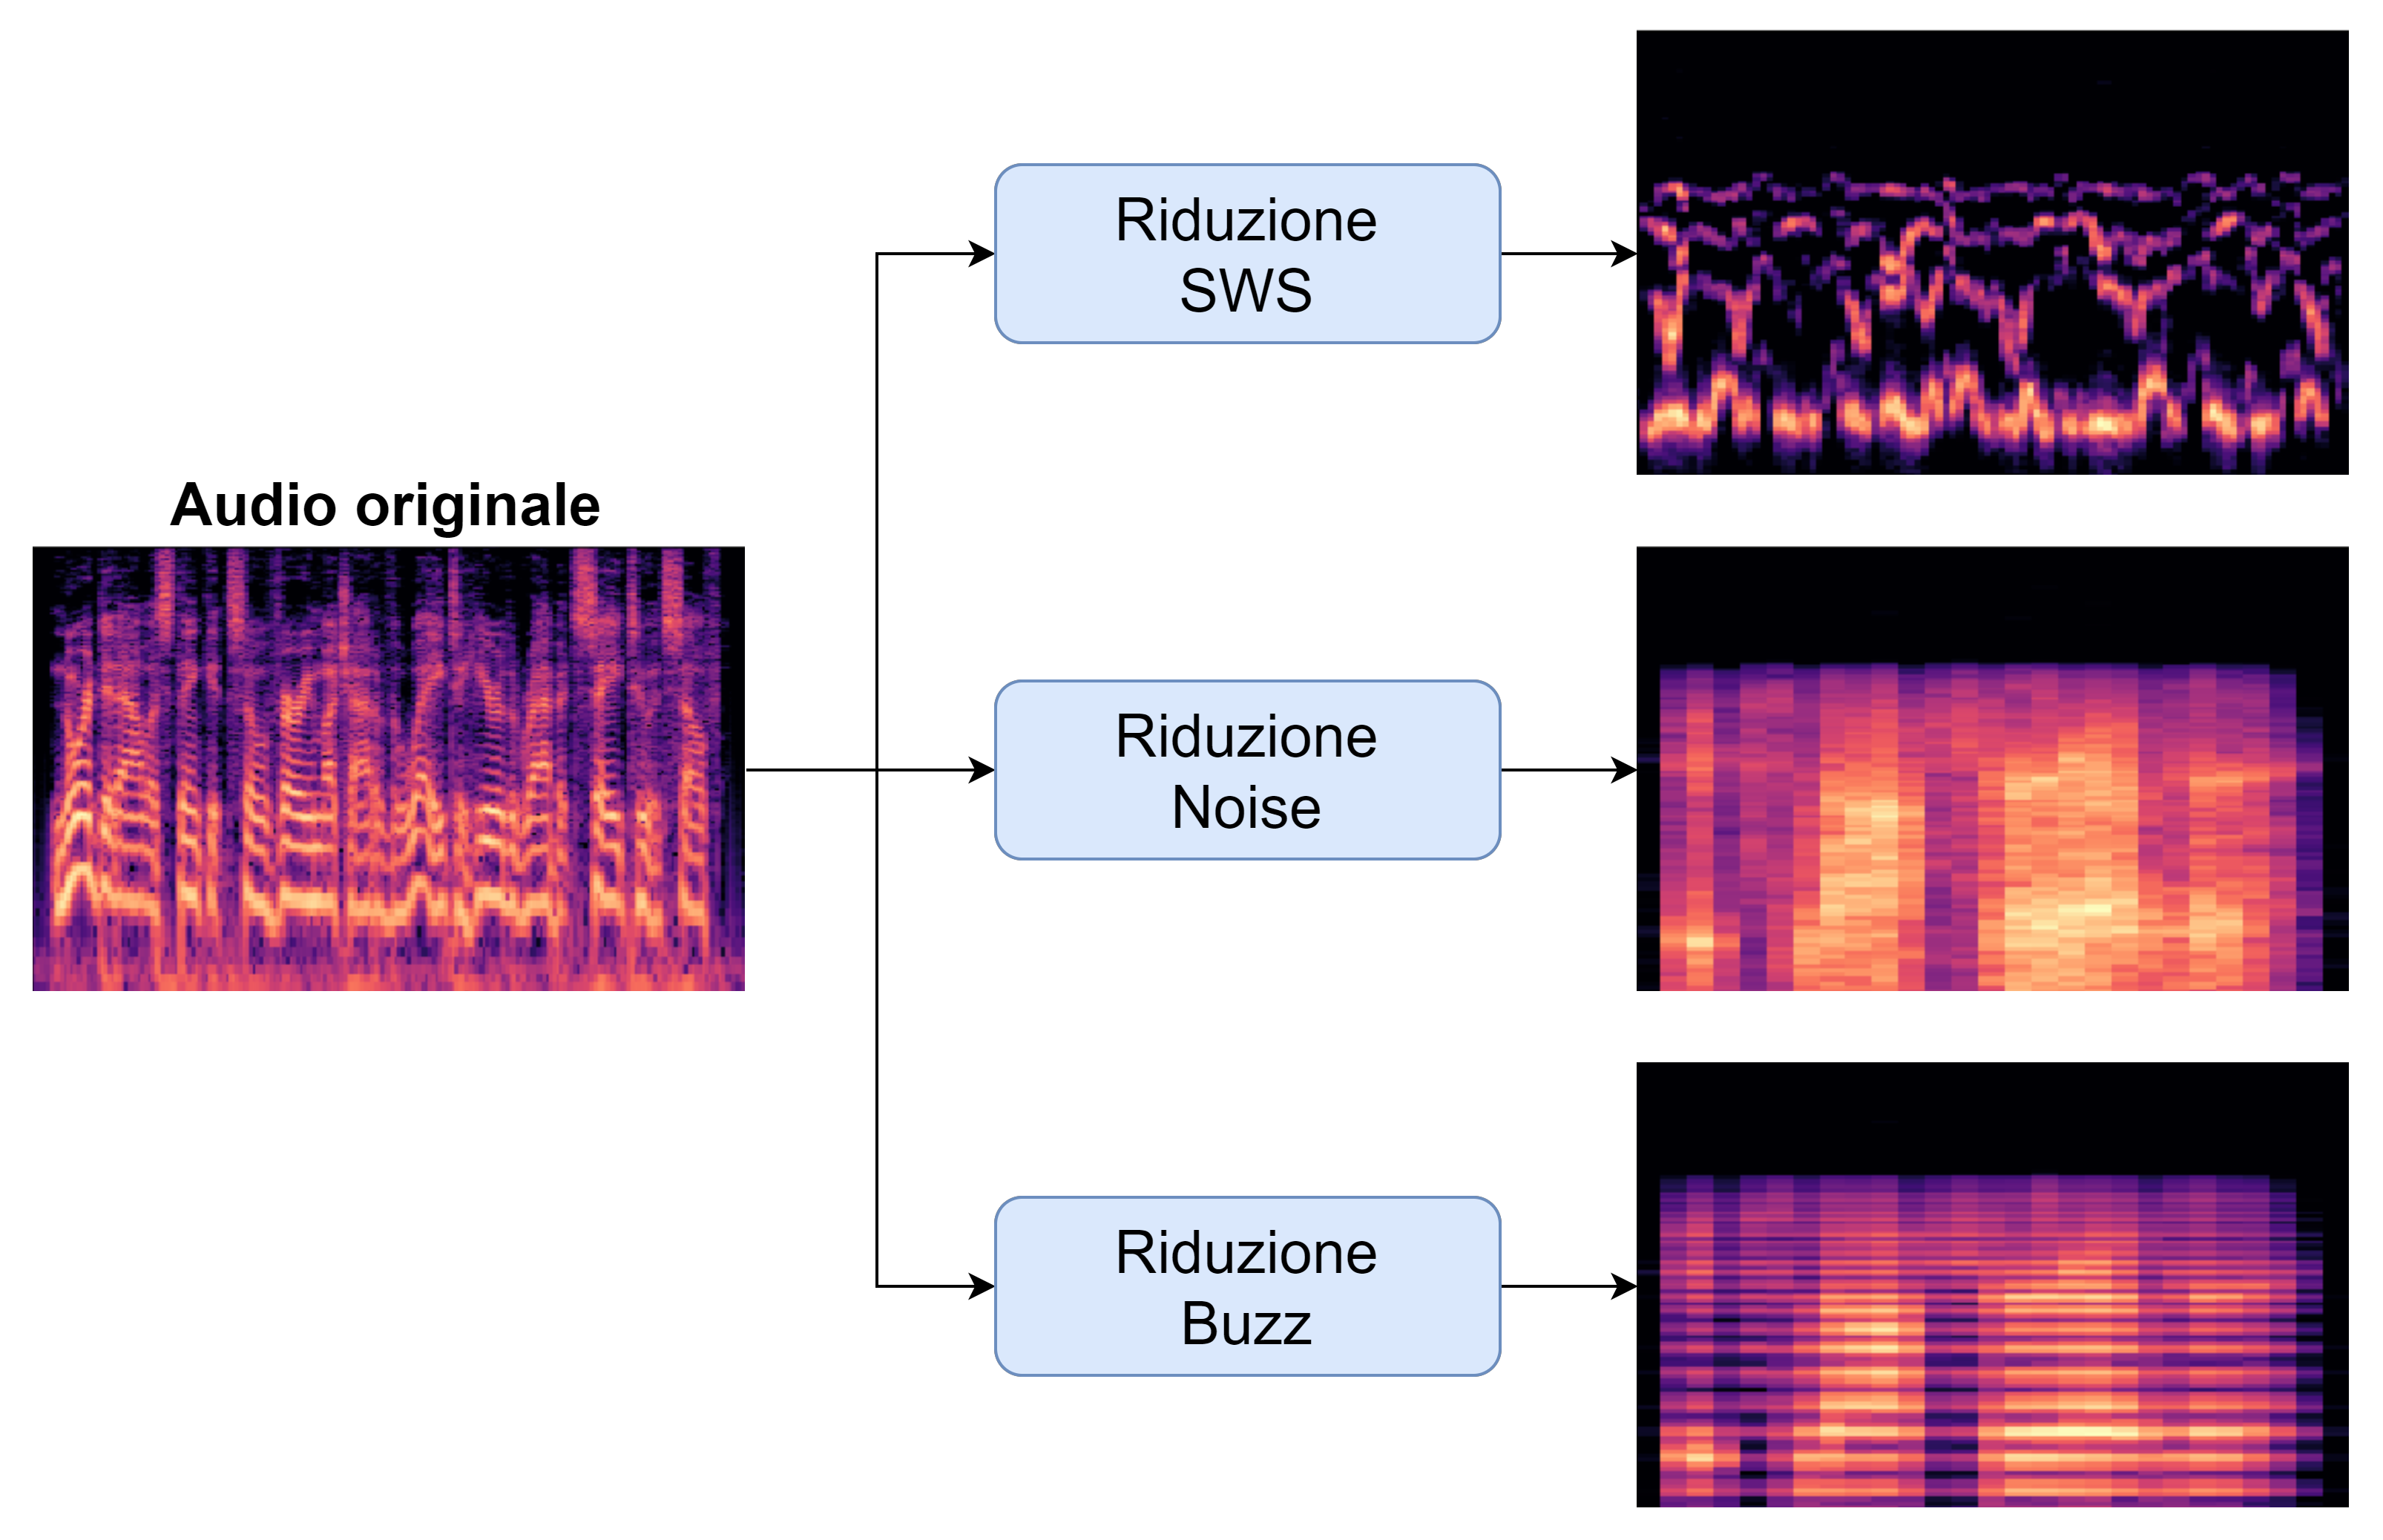
\includegraphics[width=0.8\linewidth]{figures/modulo-riduzione-spettro-sonoro}
				\caption{Risultati della riduzione dello spettro sonoro applicando i tre metodi proposti: sine-wave speech, noise vocoded speech e buzz vocoded speech.}
				\label{fig:modulo-riduzione-spettro-sonoro}
			\end{figure}
	
		\section{Modulo di conversione audio-spettrogrammi}
		Al fine di poter utilizzare la rete MaskCycleGAN-VC è necessario trasformare degli audio in spettrogrammi da fornire come input ad essa e successivamente di invertire questa trasformazione per ottenere un audio in output. È stata scelto di impiegare lo stesso modello utilizzato nel paper di riferimento di Kaneko et al.\cite{MaskCyclegan-VC}, ovvero una MelGAN\cite{melgan} pretrainata, al fine di poter effettuare un confronto più diretto sui risultati ottenuti dalle rappresentazioni scelte come input.
	
		\section{Architettura della rete}
		L'architettura della rete neurale artificiale utilizzata è la MaskCycleGAN-VC come descritta nel \autoref{chap:deep-learning} (Fig. \ref{fig:maskcyclegan-sws-vc}).		
		La scelta di non modificare parametri della rete è voluta al fine di poter ottenere dei risultati oggettivi dipendenti esclusivamente dalla riduzione spettrale proposta.
		
		\begin{figure}[h]
			\centering
			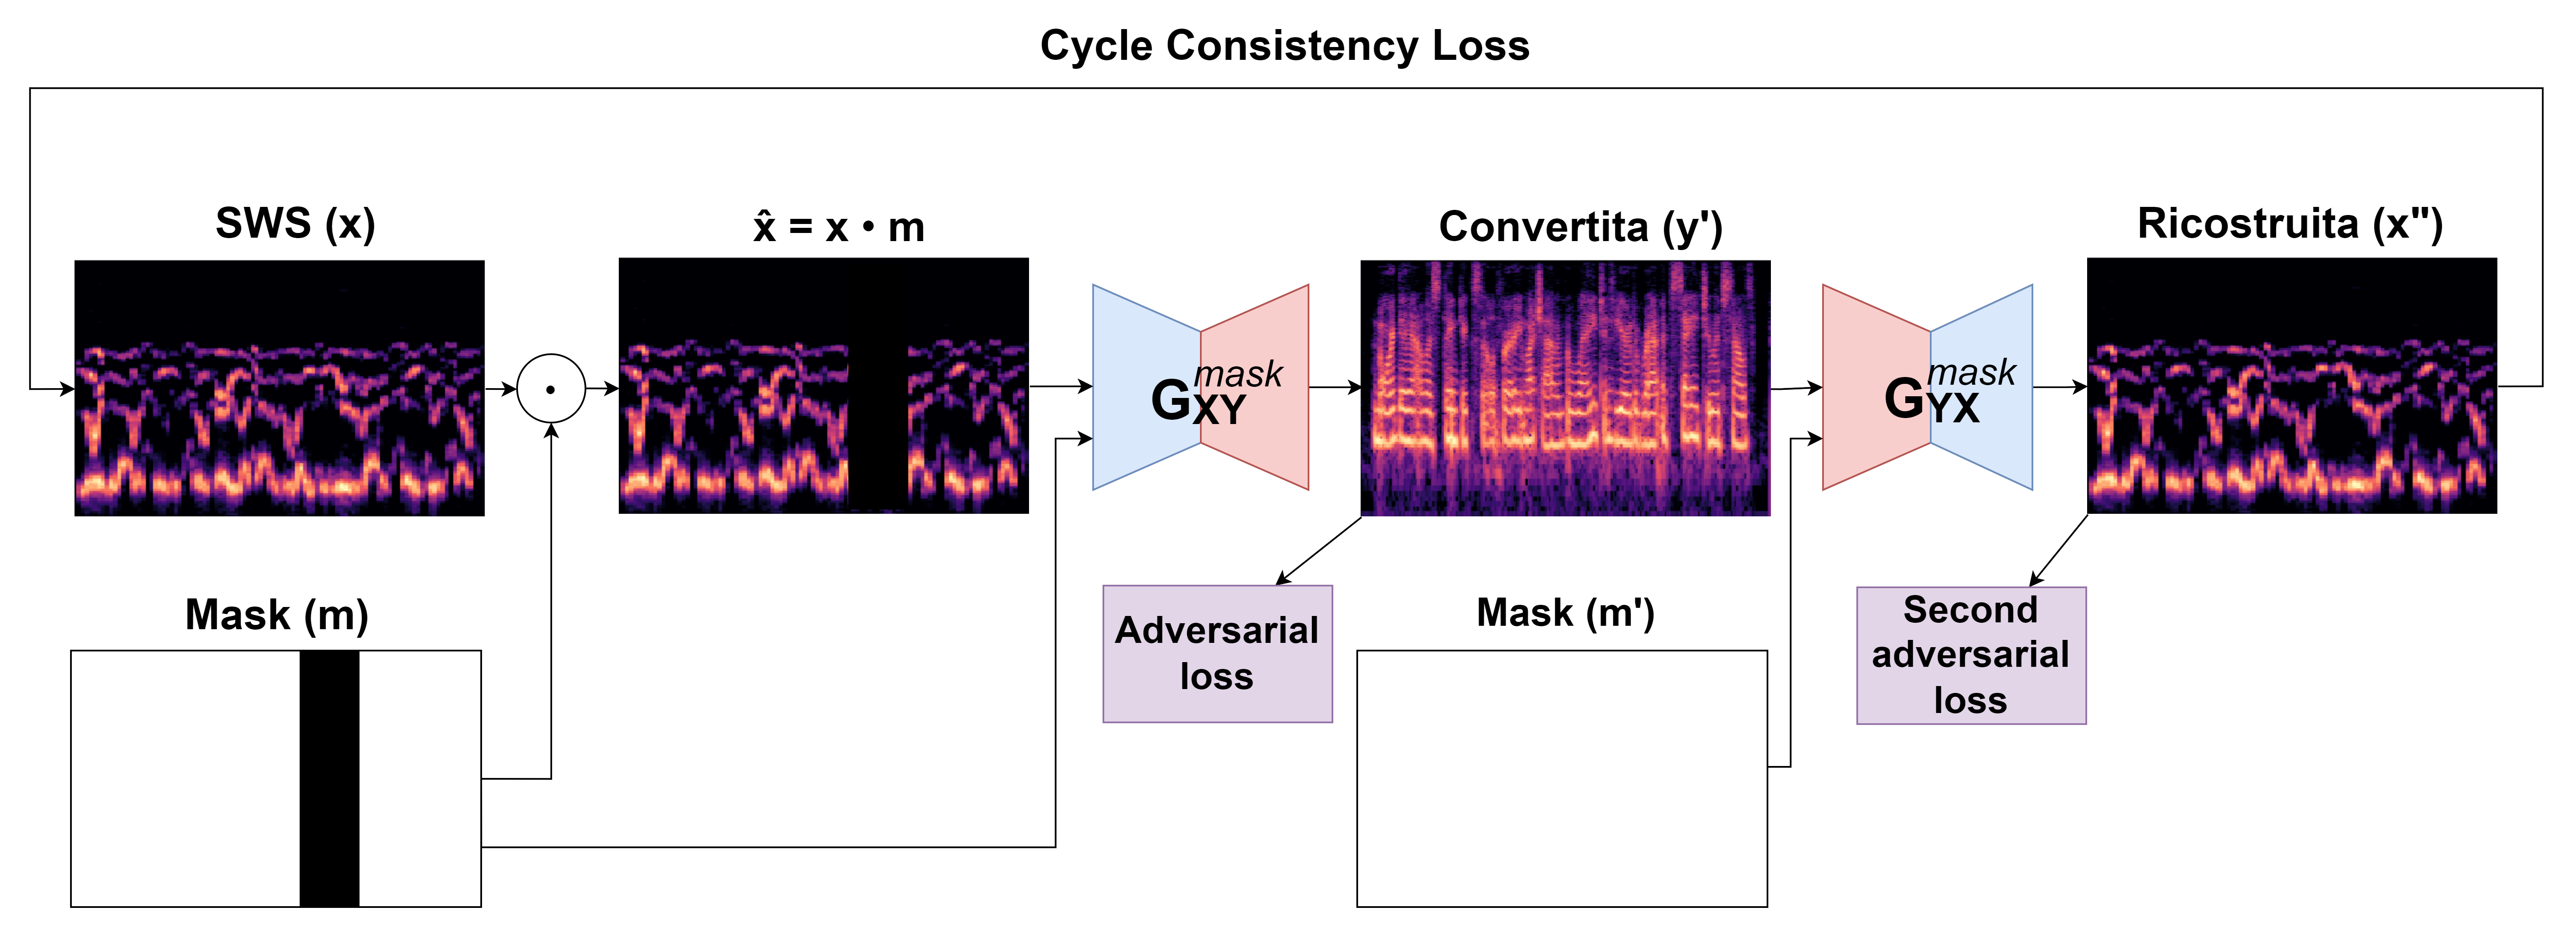
\includegraphics[width=1\linewidth]{figures/MaskCycleGAN-SWS-VC}
			\caption{Ciclo forward dell'architettura proposta impiegando il modulo di riduzione a SWS. Il modello verrà addestrato a trasformare la forma ridotta della voce di $X$ nella voce di $Y$.}
			\label{fig:maskcyclegan-sws-vc}
		\end{figure}

	
	\chapter{Test e valutazioni}
		In questo capitolo verranno descritti i test effettuati, i criteri utilizzati per la valutazione e verranno comparati le tre riduzioni spettrali proposte: SWS, noise vocoded speech e buzz vocoded speech.
		
		\section{Dataset}
		È stato utilizzato il dataset fornito dalla VCC2018 (Voice Conversion Challenge 2018) in quanto riferimento principale per le performance di voice conversion.
		
		Il dataset è formato da 8 source speaker e 4 target speaker, a ciascuno di essi corrispondono 81 audio di frasi lette (in totale circa 5 minuti di durata) con frequenza di campionamento a 22.05 kHz. Al fine di lavorare su dati non paralleli, è necessario effettuare le conversioni proposte dal task "Spoke" della VCC2018.
		
		Sono stati usati un sottoinsieme di speaker in modo da testare conversioni tra generi differenti e tra lo stesso genere, elencate a seguire:
		\begin{itemize}
			\item VCC2SF3 $\rightarrow$ VCC2TF1 (F$\rightarrow$F)
			\item VCC2SF3 $\rightarrow$ VCC2TM1 (F$\rightarrow$M)
			\item VCC2SM3 $\rightarrow$ VCC2TF1 (M$\rightarrow$F)
			\item VCC2SM3 $\rightarrow$ VCC2TM1 (M$\rightarrow$M)
		\end{itemize}
		I nomi corrispondono a quelli assegnati internamente del dataset e descrivono il genere (M, F) e l'appartenenza all'insieme di source (S) o target (T).
		
		\section{Training}
		Il dataset è stato processato come descritto nel \autoref{chap:architettura-proposta}. In particolare sono stati predisposti quattro test separati per valutare le seguenti rappresentazioni: nessuna riduzione spettrale, vocoder con noise carrier, vocoder con buzz carrier (500 Hz) e sine-wave speech con 5 formanti.
		
		Le reti sono state trainate per 150k iterazioni seguendo le specifiche della MaskCycleGAN-VC ovvero usando un ottimizzatore Adam, con learning rate impostato a 0.0002 per il generatore e 0.0001 per il discriminatore e momentum $\beta1$ e $\beta2$ rispettivamente 0.5 e 0.999. La batch size è stata impostata a 1, dove ogni sample consiste in 64 frame tagliati casualmente. La maschera applicata sull'input è stata impostata a 25.
		
		\section{Metodi di valutazione}
		Esistono varie metriche per la valutazione oggettiva della voice conversion, in questo lavoro si valuteranno come per la MaskCycleGAN-VC le seguenti: mel-cepstral distortion (MCD)\cite{mel-cepstral-distance} e Kernel DeepSpeech Distance (KDSD)\cite{kdsd}.
		
		La MCD misura la variazione di spettro, di conseguenza non è necessariamente correlata con la naturalezza del suono, mentre la KDSD misura la distanza tra le feature degli audio reali e quelli generati e ha dimostrato una correlazione con la valutazione effettuata da persone.
		Data la natura di queste misurazioni, una conversione è considerabile migliore quando queste metriche hanno risultato più basso.
		
		Verrà inoltre impiegata una MOSNet\cite{mosnet} pre-trainata per ottenere una stima di riferimento per quanto riguarda la valutazione soggettiva. Esso è un modello che, basandosi sulle opinioni reali fornite da ascoltatori alle submission effettuate alla VCC2018, è stato addestrato a predire valutazioni soggettive MOS (mean opinion score) e ha dimostrato una forte correlazione con i voti effettivi delle persone. La valutazione è espressa, come per la MOS, in una valutazione nell'intervallo [1,5] dove 1 significa una bassa qualità e 5 un'ottima qualità.
		
		\section{Risultati}
		Si riportano a seguire i risultati ottenuti dalle conversioni di voci.
		Vengono riportate le valutazioni basate sulle scale MCD, KDSD e MOSNet delle quattro conversioni effettuate per ciascuna tipologia di dati usata come input della rete.
		
		Per ogni tipologia di conversione (es. F$\rightarrow$M) sono stati messi in evidenza i risultati migliori per ciascuna metrica. Risulta interessante notare come il metodo originale \cite{MaskCyclegan-VC} senza riduzioni di spettro, ottenga ottime risultati per la metrica di KDSD, mentre le conversioni effettuate con le  riduzioni di spettro ottengono punteggi migliori per le metriche di MCD e MOSNet.
		
		\def\arraystretch{1.3}
\begin{table}[h]
	\centering
	\begin{threeparttable}
	\begin{tabular*} {\textwidth}{c @{\extracolsep{\fill}} llccc}
		\toprule
		\textbf{Riduzione spettro}\tnote{a}         & \textbf{Valutazione} & \textbf{F$\rightarrow$F} & \textbf{F$\rightarrow$M} & \textbf{M$\rightarrow$F} & \textbf{M$\rightarrow$M} \\ \hline
		\multirow{3}{*}{Nessuna riduzione \tnote{b}}        & MCD (dB) & 6.61          & 6.57          & 6.98          & 6.89          \\
		& KDSD     & \textbf{2074} & \textbf{1755} & \textbf{2770} & \textbf{1583} \\
		& MOSNet   & 3.84          & 4.46          & 3.92          & 4.58          \\ \hline
		\multirow{3}{*}{Noise vocoded\tnote{c}}     & MCD [dB] & 6.53          & \textbf{6.47} & 6.75          & 6.73          \\
		& KDSD [$\times 10^5$]     & 3269          & 2247          & 3446          & 2032          \\
		& MOSNet   & 3.90          & 4.46          & 3.89          & 4.49          \\ \hline
		\multirow{3}{*}{Buzz vocoded\tnote{c}}  & MCD [dB]             & \textbf{6.49}              & 6.49                       & \textbf{6.70}              & \textbf{6.71}              \\
		& KDSD [$\times 10^5$]     & 3063          & 2155          & 3169          & 1823          \\
		& MOSNet   & 3.80          & 4.47          & \textbf{3.94} & 4.53          \\ \hline
		\multirow{3}{*}{Sine-wave speech\tnote{c}}  & MCD [dB] & 6.55          & 6.55          & 6.98          & 6.78          \\
		& KDSD [$\times 10^5$]     & 3513          & 2621          & 4802          & 2492          \\
		& MOSNet   & \textbf{3.91} & \textbf{4.48} & 3.86          & \textbf{4.61} \\
		\bottomrule
	\end{tabular*}
	\begin{tablenotes}
		\item[a] Modulo di riduzione dello spettro applicato sui dati di input.
		\item[b] Nessuna riduzione spettrale applicata, modello trainato come proposta da Kaneko et al. in \cite{MaskCyclegan-VC}.
		\item[c] Metodi di riduzione spettrale proposti, come descritti nella \autoref{sec:proposta-riduzione}.
	\end{tablenotes}
\end{threeparttable}
\end{table}


	\chapter{Conclusioni}
	In questo lavoro si sono combinate tecniche di speech processing più tradizionali con le odierne di deep learning al fine di ricercare una forma a spettro ridotto della voce che permetta di ridurre la componente acustica, preservando quella linguistica.
	
	Dalle valutazioni si evince che questo approccio è possibile e che i suoi risultati sono equiparabili a quelli ottenuti usando audio senza riduzioni di spettro. Come sviluppi futuri si ritiene interessante approfondirne l'applicazione in altri campi, come ad esempio nella speech recognition al fine di addestrare modelli anonimizzati, e sviluppare metodi per sfruttare al meglio questa forma facilmente manipolabile per data augmentation.
	
	
	\backmatter

	\cleardoublepage
	\phantomsection % Give this command only if hyperref is loaded
	\addcontentsline{toc}{chapter}{\bibname}
	% Here put the code for the bibliography. You can use BibTeX or
	% the BibLaTeX package or the simple environment thebibliography.
	\bibliographystyle{plain} % We choose the "plain" reference style
	\bibliography{tesi} % Entries are in the tesi
\end{document}